\documentclass[letterpaper, 12pt]{article}
\usepackage{standalone}

\usepackage{geometry}
 \geometry{
 letterpaper,
 total={170mm,257mm},
 left=20mm,
 top=20mm,
 bottom=20mm
 }
\usepackage{graphicx} % Required for inserting images
\usepackage{authblk}
\usepackage{amssymb}
\usepackage{lipsum}
\usepackage{float}
\usepackage{times}
\usepackage{amsmath}
\usepackage[format=plain,
            labelfont={bf,it},
            textfont=it]{caption}
\captionsetup{justification=raggedright,singlelinecheck=false}
\usepackage{ragged2e}
\usepackage{longtable}
\usepackage{comment}
\usepackage{setspace}
\usepackage{fancyhdr}
\usepackage{titlesec}
\usepackage[hyperindex,breaklinks]{hyperref}
\hypersetup{
    colorlinks=true,
    linkcolor=blue,
    filecolor=magenta,      
    urlcolor=blue,
    pdftitle={Overleaf Example},
    pdfpagemode=FullScreen,
    }
% \usepackage{background} % add COSIG logo to page
\usepackage[T1]{fontenc}
\usepackage{helvet}
\renewcommand{\familydefault}{\sfdefault}
\pagenumbering{arabic}
\usepackage[skip=10pt plus1pt, indent=40pt]{parskip}

\begin{comment}
\backgroundsetup{
   scale=1,
   angle=0,
   opacity=1,
   color=black,
   contents={\begin{tikzpicture}[remember picture, overlay]
      \node at ([xshift=3cm,yshift=1cm] current page.south west)
            {
\includegraphics[width = 5cm]{img/home/241017_final_logo_mockup.png}}; %<- change the name of image
     \end{tikzpicture}}
 }
\end{comment}

\titlespacing*{\section}
{0pt}{1.5ex plus 1ex minus .2ex}{1.3ex plus .2ex}

\renewcommand\Authfont{\fontsize{12}{14.4}\selectfont}
\renewcommand\Affilfont{\fontsize{9}{10.8}\itshape}

\begin{document}

\documentclass[letterpaper, 12pt]{article}

\usepackage{geometry}
 \geometry{
 letterpaper,
 total={170mm,257mm},
 left=20mm,
 top=20mm,
 bottom=20mm
 }
\usepackage{graphicx} % Required for inserting images
\usepackage{authblk}
\usepackage{amssymb}
\usepackage{lipsum}
\usepackage{float}
\usepackage{times}
\usepackage{amsmath}
\usepackage[format=plain,
            labelfont={bf,it},
            textfont=it]{caption}
\captionsetup{justification=raggedright,singlelinecheck=false}
\usepackage{ragged2e}
\usepackage{longtable}
\usepackage{comment}
\usepackage{setspace}
\usepackage{fancyhdr}
\usepackage{titlesec}
\usepackage[hyperindex,breaklinks]{hyperref}
\hypersetup{
    colorlinks=true,
    linkcolor=blue,
    filecolor=magenta,      
    urlcolor=blue,
    pdftitle={Overleaf Example},
    pdfpagemode=FullScreen,
    }
% \usepackage{background} % add COSIG logo to page
\usepackage[T1]{fontenc}
\usepackage{helvet}
\renewcommand{\familydefault}{\sfdefault}
\pagenumbering{gobble}
\usepackage[skip=10pt plus1pt, indent=40pt]{parskip}
\usepackage{orcidlink}

\begin{comment}
\backgroundsetup{
   scale=1,
   angle=0,
   opacity=1,
   color=black,
   contents={\begin{tikzpicture}[remember picture, overlay]
      \node at ([xshift=3cm,yshift=1cm] current page.south west)
            {
\includegraphics[width = 5cm]{img/home/241017_final_logo_mockup.png}}; %<- change the name of image
     \end{tikzpicture}}
 }
\end{comment}

\titlespacing*{\section}
{0pt}{1.5ex plus 1ex minus .2ex}{1.3ex plus .2ex}

\renewcommand\Authfont{\fontsize{12}{14.4}\selectfont}
\renewcommand\Affilfont{\fontsize{9}{10.8}\itshape}


\begin{document}
\flushleft

\includegraphics[width=\textwidth]{img/home/241017_final_logo_mockup.png}

\section*{Anyone can do post-publication peer review.}
\section*{Anyone can be a steward of the scientific literature.}
\section*{Anyone can do forensic metascience.}
\section*{Anyone can sleuth.}

However, investigating the integrity of the published scientific literature often requires domain-specific knowledge that not everyone will have. This open source project is a collection of guides written and maintained by publication integrity experts to distribute this domain-specific knowledge so that others can participate in post-publication peer review.

COSIG currently hosts 17 guides and was last updated on 4 April 2025.

Except where otherwise indicated, all material in COSIG is available under a \href{https://creativecommons.org/licenses/by-nc-sa/4.0/deed.en}{CC BY-NC-SA 4.0 license}. That means that you are free to distribute, remix, adapt, and build upon the material in any medium or format for noncommercial purposes only, and only so long as COSIG is properly cited. If you remix, adapt, or build upon the material, you must license the modified material under identical terms.

Suggestions to improve COSIG can be submitted by opening an issue on \href{https://github.com/reeserich/cosig/issues}{COSIG's GitHub repo}.


\includegraphics[width=0.2\textwidth]{img/home/Cc-by-nc-sa_icon.svg.png}

\begin{comment}
\pagebreak

\section*{Table of contents}

\subsection*{General guides}

\begin{itemize}
    \setlength\itemsep{-0.5em}
    \item PubPeer commenting - best practices
    \item Extracting vector graphics from a PDF
    \item The vertical line test
    \item Software for image forensics
\end{itemize}

\subsection*{Biology and medicine}

\begin{itemize}
    \setlength\itemsep{-0.5em}
    \item Misidentified and non-verifiable cell lines
\end{itemize}

\subsection*{Materials science and engineering}

\begin{itemize}
    \setlength\itemsep{-0.5em}
    \item Energy-dispersive X-ray spectroscopy
    \item X-ray diffraction patterns - Scherrer's equation
\end{itemize}

\subsection*{Mathematics and statistics}

\begin{itemize}
    \setlength\itemsep{-0.5em}
    \item Standard deviation versus standard error
\end{itemize}
\end{comment}

\pagebreak

The following individuals have contributed to COSIG in some way:

\begin{itemize}
    \setlength\itemsep{-0.5em}
    \item Ren\'e Aquarius \orcidlink{0000-0002-0968-6884}
    \item David Bimler \orcidlink{0000-0003-2405-0697}
    \item Jennifer Byrne \orcidlink{0000-0002-8923-0587}
    \item Jana Christopher \orcidlink{0000-0002-2699-3368}
    \item M.V. Dougherty \orcidlink{0000-0002-8731-6045}
    \item Yagmur Ozturk \orcidlink{0000-0002-2843-8990}
    \item Kevin Patrick \orcidlink{0009-0001-7491-9242}
    \item Solal Pirelli \orcidlink{0009-0003-4336-1316}
    \item Reese Richardson \orcidlink{0000-0002-6058-5886}, \textbf{Maintainer}
\end{itemize}

\end{document}

\tableofcontents

\makeatletter
\addtocontents{toc}{\let\Hy@linktoc\Hy@linktoc@none}
\makeatother

\documentclass[letterpaper, 12pt]{article}

\usepackage{geometry}
 \geometry{
 letterpaper,
 total={170mm,257mm},
 left=20mm,
 top=20mm,
 bottom=20mm
 }
\usepackage{graphicx} % Required for inserting images
\usepackage{authblk}
\usepackage{amssymb}
\usepackage{lipsum}
\usepackage{float}
\usepackage{times}
\usepackage{amsmath}
\usepackage[format=plain,
            labelfont={bf,it},
            textfont=it]{caption}
\captionsetup{justification=raggedright,singlelinecheck=false}
\usepackage{ragged2e}
\usepackage{longtable}
\usepackage{comment}
\usepackage{setspace}
\usepackage{fancyhdr}
\usepackage{titlesec}
\usepackage[hyperindex,breaklinks]{hyperref}
\hypersetup{
    colorlinks=true,
    linkcolor=blue,
    filecolor=magenta,      
    urlcolor=blue,
    pdftitle={Overleaf Example},
    pdfpagemode=FullScreen,
    }
% \usepackage{background} % add COSIG logo to page
\usepackage[T1]{fontenc}
\usepackage{helvet}
\renewcommand{\familydefault}{\sfdefault}
\pagenumbering{gobble}
\usepackage[skip=10pt plus1pt, indent=40pt]{parskip}

\begin{comment}
\backgroundsetup{
   scale=1,
   angle=0,
   opacity=1,
   color=black,
   contents={\begin{tikzpicture}[remember picture, overlay]
      \node at ([xshift=3cm,yshift=1cm] current page.south west)
            {
\includegraphics[width = 5cm]{img/home/241017_final_logo_mockup.png}}; %<- change the name of image
     \end{tikzpicture}}
 }
\end{comment}

\titlespacing*{\section}
{0pt}{1.5ex plus 1ex minus .2ex}{1.3ex plus .2ex}

\renewcommand\Authfont{\fontsize{12}{14.4}\selectfont}
\renewcommand\Affilfont{\fontsize{9}{10.8}\itshape}
 
\begin{document}
\flushleft

\includegraphics[width=0.5\textwidth]{img/home/241017_final_logo_mockup.png}

\section*{Misidentified and non-verifiable cell lines}
\textit{Last updated: 5 February 2025}
\subsection*{Cell lines}

A cell line is a population of cells that can be grown in a laboratory culture indefinitely. Cell lines are an essential tool for biomedical research because they allow biological experiments to be performed in vitro (i.e. outside of a living organism). For instance, researchers developing new cancer drugs will certainly test the effect of their drug candidates on many different cancer cell lines before ever considering testing the drug candidate on live animals, let alone human patients.

Because cell lines can grow indefinitely, one research laboratory or laboratory supplier can take a few cells from their cell line stock and give them to another laboratory for that laboratory to begin culturing their own stock. By far the most popular cell line is HeLa, and the many thousands of \href{https://www.cellosaurus.org/CVCL_0030}{HeLa cell stocks} used in biomedical research around the world can all be traced back to the original stock of "immortal" cervical cancer cells taken from \href{https://en.wikipedia.org/wiki/Henrietta_Lacks}{Henrietta Lacks in 1951}.

\subsection*{Misidentified/contaminated cell lines}

One complication of relying on cell lines for biomedical research is that stocks will often become cross-contaminated by other cell lines. For instance, HeLa is extremely aggressive as cancer cell lines go and HeLa cells will easily overtake other cell line stocks that are stored nearby. The popular gastric cancer cell line \href{https://www.cellosaurus.org/CVCL_3360}{BGC-823} is one such victim of HeLa’s aggression; there are no remaining uncontaminated stocks of BGC-823 and thus it is no longer considered an appropriate experimental model for gastric cancer.


\begin{figure}[h!tbp]
    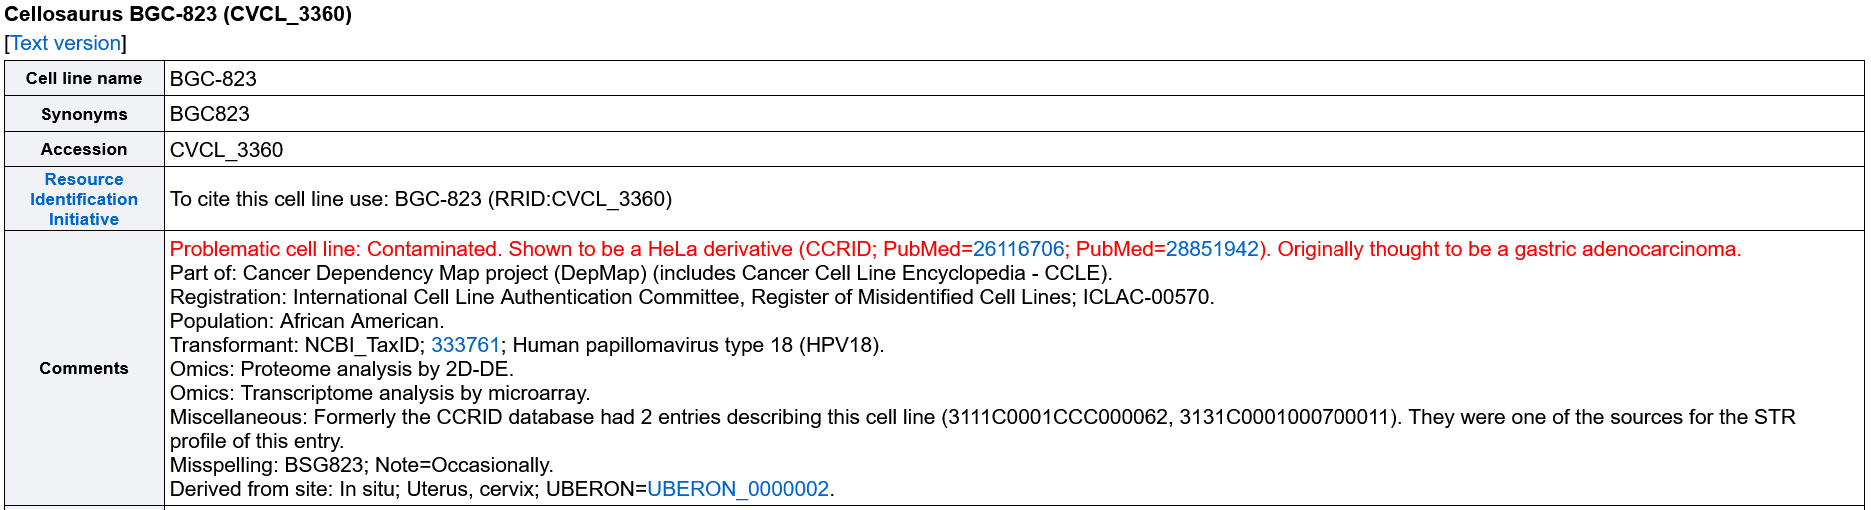
\includegraphics[width=\textwidth]{img/cell_lines/Screenshot 2024-11-04 at 11-59-23 Cellosaurus cell line BGC-823 (CVCL_3360).png}
    \caption*{The Cellosaurus entry for \href{https://www.cellosaurus.org/CVCL_3360}{BGC-823} now warns about the cell line being contaminated by HeLa.}
\end{figure}

The International Cell Line Authentication Committee maintains \href{https://iclac.org/databases/cross-contaminations/}{a register of misidentified cell lines} that is currently 593 entries long. A good number of these cell lines were contaminated by cells from a completely different organism, such as human salivary gland cell line \href{https://www.cellosaurus.org/CVCL_6883}{CAC2}, which is actually made up of unknown cells from a rat.

\href{https://www.cellosaurus.org/index.html}{Cellosaurus} is an encyclopedia of thousands of cell lines and will link to studies showing that a cell line is contaminated or otherwise misidentified.

Because different cell lines can have a wide variety of responses to the same treatment, it is essential that researchers avoid misidentified cell lines and only work with authenticated cell lines that actually represent their system of interest. Consider the fact that cancer cell lines can have wildly different sensitivity to the chemotherapy drug \href{https://www.cancerrxgene.org/compound/Paclitaxel/11/overview/ic50?tissue=PANCANCER&screening_set=GDSC1}{paclitaxel}.

\begin{figure}[h!tbp]
    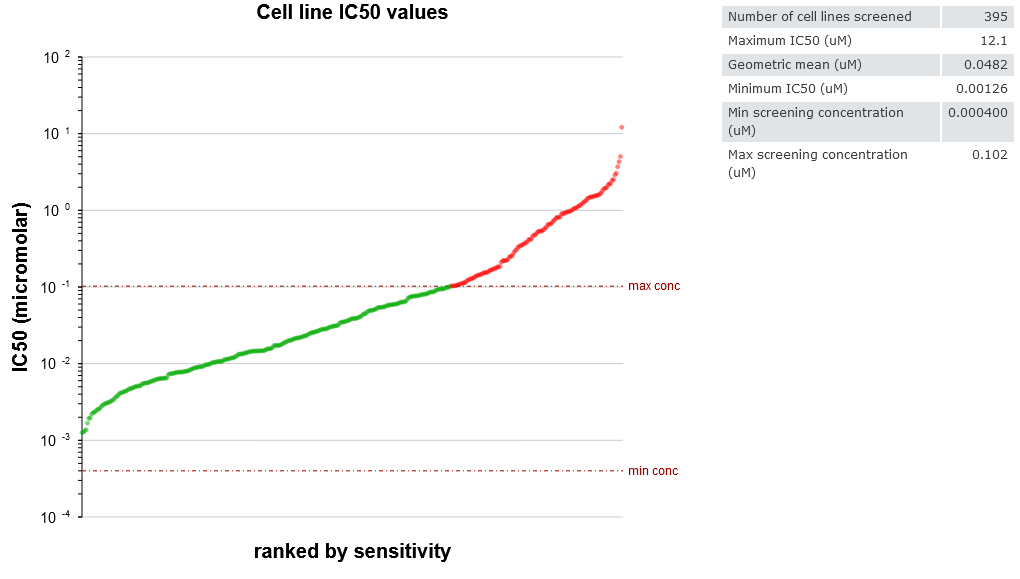
\includegraphics[width=\textwidth]{img/cell_lines/Screenshot 2024-11-04 at 12-02-27 Drug Paclitaxel - Cancerrxgene - Genomics of Drug Sensitivity in Cancer.png}
    \caption*{\href{https://en.wikipedia.org/wiki/IC50}{Half-maximal inhibitory concentration (IC50)}, in this context, is a measure that describes what concentration of a drug is needed to inhibit the growth of a cell line by 50\%. The \href{https://www.cancerrxgene.org/compound/Paclitaxel/11/overview/ic50?tissue=PANCANCER&screening_set=GDSC1}{Genomics of Drug Sensitivity in Cancer (GDSC) database} estimated these values for 395 cell lines for the drug paclitaxel. Note that paclitaxel can be more than a thousand times as potent against some cell lines than others, even for cell lines from the same type of cancer.}
\end{figure}

\subsection*{Cell line verification/authentication}

Researchers should always verify that their cell lines stocks are what they believe them to be. There are a number of ways researchers can verify the integrity of their cell line stocks (many of which are \href{https://www.atcc.org/resources/technical-documents/cell-line-authentication-test-recommendations}{detailed by the American Type Culture Collection}). The most common authentication technique is \href{https://en.wikipedia.org/wiki/STR_analysis}{short tandem repeat (STR) profiling}, which identifies specific molecular signatures in a cell line's genome.

\subsection*{Non-verifiable cell lines}

The names of cell lines are usually just a jumble of letters and numbers and thus can often be easily confused. For instance, the name of \href{https://www.cellosaurus.org/CVCL_3360}{BGC-823} is very similar to that of \href{https://www.cellosaurus.org/CVCL_5334}{MGC-803}, another misidentified gastric cancer cell line. One might easily misspell these cell lines as "BGC-803" or "MGC-823". However, it was recently reported by \href{https://doi.org/10.1002/ijc.34995}{Oste et al. (2024)} that many publications will use these misspelled identifiers to refer to another cell line entirely distinct from these existing cell lines. For instance, \href{https://doi.org/10.1002/jgm.3330}{Zhong et al. (2021)} report experiments in cell lines "BGC-803" and "BSG-823" in addition to experiments in the contaminated cell lines BGC-823 and MGC-803.

Hundreds of articles have referred to experiments in these cell lines despite there being no indication that these cell lines actually exist; there are no entries for these cell lines in any cell line indices, they cannot be found in any supplier catalogs, there are no articles describing how these cell lines were established and no one seems to have produced any genetic profiles of these cell lines to confirm their identities. Oste et al. identified eight such "miscellings": BGC-803, BSG-803, BSG-823, GSE-1, HGC-7901, HGC-803, MGC-823 and TIE-3, although there are certainly many more that have not been studied in detail.

\subsection*{Example 1: Contaminated cell lines}

\href{https://doi.org/10.1016/j.yexcr.2017.09.005}{Liu et al. (2017)} report experiments in the cell lines \href{https://www.cellosaurus.org/CVCL_5334}{MGC-803}, \href{https://www.cellosaurus.org/CVCL_6926}{L02} and \href{https://www.cellosaurus.org/CVCL_0534}{SMMC-7721}. However, each of these cell lines are contaminated by HeLa are thus are no longer considered suitable models for their respective cancers.

\subsection*{Example 2: Non-verifiable and contaminated cell lines}

\href{https://doi.org/10.1186/s12943-018-0874-1}{Yang et al. (2018)} mention and provide experimental results in 10 different cell lines, of which 4 are problematic, shown below in bold:

\begin{itemize}
    \setlength\itemsep{-0.5em}
    \item \textbf{SUN-216}: mentioned once in text of paper and again in Figure 1B, both spelled as SUN-216. SNU-216 is an existing cell line. A possible non-verifiable cell line identifier, but not one that has yet been studied in depth.
    \item \textbf{BGC-823}: Contaminated cell line.
    \item AGS
    \item \textbf{BGC-803}: Mentioned once in text and again in Figure 1B. One of the eight non-verifiable cell line identifiers studied by Oste et al. Likely derived from a typo that confused the cell lines MGC-803 and BGC-823, both contaminated.
    \item NUGC4
    \item MKN74
    \item MKN45
    \item \textbf{SGC-7901}: Contaminated cell line.
    \item HGC-27
    \item GES-1
\end{itemize}

\subsection*{Additional resources}

\begin{itemize}
    \setlength\itemsep{-0.5em}
    \item \href{https://www.atcc.org/resources/technical-documents/cell-line-authentication-test-recommendations}{ATCC Cell Line Authentication Test Recommendations}
    \item \href{https://www.cellosaurus.org/index.html}{Cellosaurus}
    \item \href{https://iclac.org/}{International Cell Line Authentication Committee (ICLAC)}
    \item \href{https://iclac.org/references/reading-reviews/}{ICLAC-curated reviews on cell line misidentification}
    \item \href{https://doi.org/10.1002/ijc.34995}{"Misspellings or 'miscellings'—Non-verifiable and unknown cell lines in cancer research publications" (2024)}

\end{itemize}


\end{document}
\documentclass[letterpaper, 12pt]{article}

\usepackage{geometry}
 \geometry{
 letterpaper,
 total={170mm,257mm},
 left=20mm,
 top=20mm,
 bottom=20mm
 }
\usepackage{graphicx} % Required for inserting images
\usepackage{authblk}
\usepackage{amssymb}
\usepackage{lipsum}
\usepackage{float}
\usepackage{times}
\usepackage{amsmath}
\usepackage[format=plain,
            labelfont={bf,it},
            textfont=it]{caption}
\captionsetup{justification=raggedright,singlelinecheck=false}
\usepackage{ragged2e}
\usepackage{longtable}
\usepackage{comment}
\usepackage{setspace}
\usepackage{fancyhdr}
\usepackage{titlesec}
\usepackage[hyperindex,breaklinks]{hyperref}
\hypersetup{
    colorlinks=true,
    linkcolor=blue,
    filecolor=magenta,      
    urlcolor=blue
    }
% \usepackage{background} % add COSIG logo to page
\usepackage[T1]{fontenc}
\usepackage{helvet}
\renewcommand{\familydefault}{\sfdefault}
\pagenumbering{gobble}
\usepackage[skip=10pt plus1pt, indent=40pt]{parskip}

\begin{comment}
\backgroundsetup{
   scale=1,
   angle=0,
   opacity=1,
   color=black,
   contents={\begin{tikzpicture}[remember picture, overlay]
      \node at ([xshift=3cm,yshift=1cm] current page.south west)
            {
\includegraphics[width = 5cm]{img/home/241017_final_logo_mockup.png}}; %<- change the name of image
     \end{tikzpicture}}
 }
\end{comment}

\titlespacing*{\section}
{0pt}{1.5ex plus 1ex minus .2ex}{1.3ex plus .2ex}

\renewcommand\Authfont{\fontsize{12}{14.4}\selectfont}
\renewcommand\Affilfont{\fontsize{9}{10.8}\itshape}
 
\begin{document}
\flushleft

\includegraphics[width=0.5\textwidth]{img/home/241017_final_logo_mockup.png}

\section*{Citations}
\addcontentsline{toc}{section}{Citations}
\textit{Last updated: 4 May 2025}

Science is built incrementally, one discovery at a time.
Scientific articles \emph{cite} other articles to make reference to previous work and claims.
\emph{Citations} are a core feature of all scientific papers.

Citations are typically short references in an article's text to entries in a ``References'' or ``Bibliography'' section,
which itself contains paper titles, author names, years, and so on.
Different journals and publishers adopt different \href{https://libguides.brown.edu/citations/styles}{styles of citations}, typically either numeric (e.g., ``[1]'', ``[42]'')
or author-year (e.g., ``[Smith 2024]'', ``[Garcia 1974b]''). Authors often cite multiple sources at once (e.g., ``Several studies have found that the $A$ is positively correlated with $B$ [Smith 2024, Rodriguez 2023, Wang 2022]'').

Counting the number of times an article has been cited is an imperfect measure of how influential an article might be since it usually indicates that others found at least some part of the paper useful or otherwise built upon the work described in the article.

Citation counting is also often used to measure the impact and influence of authors. For instance, authors are often judged by their \href{https://doi.org/10.1073%2Fpnas.0507655102}{$h$-index}.
Someone with an $h$-index of $N$ has published $N$ articles each cited at least $N$ times. Similarly, journals are often evaluated by how often the articles they publish are cited, such as through the \href{https://doi.org/10.1001%2Fjama.295.1.90}{journal impact factor (JIF)}. JIF roughly corresponds to the average number of citations each article receives within a certain time frame following publication. The only official source for JIF is \href{https://clarivate.com/academia-government/scientific-and-academic-research/research-funding-analytics/journal-citation-reports/}{Clarivate's Journal Citation Reports}, which uses the database \href{https://clarivate.com/academia-government/scientific-and-academic-research/research-discovery-and-referencing/web-of-science/}{Web of Science}.

Heuristics like $h$-index and JIF are \href{https://doi.org/10.1038/d41586-022-02984-2}{used frequently in academic hiring and promotion decisions} as proxies of researcher productivity and influence. As a result, it is generally desirable for academics to acquire a higher number of citations than their peers. Similarly, journal editors and publishers may seek to increase the number of citations to their journals' articles to augment their journals' reputations.

\subsection*{Expected citation behavior}

Any claim that is not ``common sense'' or ``common knowledge'' generally requires a citation, although this is context-dependent.
Citations can reference a specific claim from a source (e.g., ``Less than 40\% of frobnicators are red [Zhang 2003]''). 
Citations can also point to a previous work as an example (e.g. ``We measure frobnication using the standard XYZ technique [24]'').
For basic claims that would be common knowledge among an article's likely readers (e.g., ``DNA is double-stranded'' or ``computers use binary digits'')
no citation is necessary.

\subsection*{Problematic citation behavior}

Citations can be problematic for a number of reasons. Some problematic citations behaviors are quite common and may not represent intentional distortions. For instance, authors may claim something about a cited article that is untrue or is unsupported by the cited article's text. On the other hand, other problematic citation behaviors are the direct result of \href{https://doi.org/10.24318/cope.2019.3.1}{citation manipulation} intended to inflate the previously-described citation metrics.

\subsection*{Archetypes of common problematic citation behaviors}

This section describes common issues that can be found among an article's citations, as well as possible motivations and explanations for these issues. Relevant examples are provided for each. Note that these behaviors are not mutually exclusive.

\subsubsection*{Missing citations}

When making claims or showing data that was not the result of the authors' original research work, authors should cite their sources. Often, this does not actually occur.

(\href{https://pubpeer.com/publications/8A2CF2E1EBFD3ADCD835ADB91DDFE8}{example})

\subsubsection*{Citations that do not accurately reflect the content of the cited article}

Statements containing citations often do not accurately reflect what is actually contained in the cited article. It is commonplace (but nonetheless problematic) for authors to \href{https://ori.hhs.gov/citing-sources-were-not-read-or-thoroughly-understood}{cite articles that they haven't actually thoroughly read}.

(\href{https://pubpeer.com/publications/6E8756FAB18C392065D8313D271090}{example 1}, \href{https://pubpeer.com/publications/D3E493ADF94B3031D24C280F54F37E}{example 2})

\subsubsection*{Many citations at once}

More than a handful of citations to back up a single statement can be excessive. This practice can be especially problematic if these blocks of citations contain many citations to the same author or are mostly irrelevant to the statement being made.

(\href{https://pubpeer.com/publications/D6A50C6DD455715DE626C1CC56B8EB}{example 1}, \href{https://pubpeer.com/publications/11C10949E0FF4EA3C31B6A45F4E22C}{example 2})

\subsubsection*{Many citations to the same author}

More than a handful of citations to the same author in a paper is unusual. This can occur naturally if most of the previous scholarship on a topic is by the same author. However, this can also be an indication of a deliberate effort to inflate particular authors' citation metrics. 

(\href{https://pubpeer.com/publications/0C7C1F371CB05161EEACC303692521}{example})

\subsubsection*{Many self-citations}

Consistently citing the authors' own papers is problematic. Most citation metrics explicitly exclude self-citations.

(\href{https://pubpeer.com/publications/3EAC0C5735F8D48FF1D4B06C6BFC30}{example})

\subsubsection*{Unused citations}

Citations are typically expected to be used in the paper's main text, so references that only appear in an article's bibliography can be suspicious.

(\href{https://pubpeer.com/publications/0C7E7F2703724338046FF2A0AA8392}{example})

\subsubsection*{Overly specific citations}

Citing very specific applications of a concept instead of a definition or review of the concept is strange, especially for fundamental concepts.

(\href{https://pubpeer.com/publications/5A064B2F4AE7F13D6E1F559F84492F}{example})

\subsubsection*{Unrelated/irrelevant citations}

Citing articles that have nothing to do with the statement for which they are cited (\emph{citation context}) is inherently problematic.

(\href{https://pubpeer.com/publications/B9CE2B145B02E439BA9C5B2C2D5F12}{example 1}, \href{https://pubpeer.com/publications/C21D670DD4C94B02C78809A55ED385}{example 2})

\subsubsection*{``Suggested'' citation batches}

Reviewers who consistently ask authors to cite many of the reviewer's papers are, at best, in an ethical gray area. Authors will often include reviewers' and editors' suggested citations in the hopes of passing through peer review.

(\href{https://pubpeer.com/publications/90719DBC6E5FF2AC32FDE74F1A6A7F}{example 1}, \href{https://pubpeer.com/publications/1924F147DE045B97261004EB2387AE}{example 2})

\subsubsection*{Citation magnets}

The same paper cited in irrelevant or barely relevant contexts across many papers,
especially within the same venue, is an indication something is deeply wrong.  Such ``citation magnets'' are often cited alongside other citation magnets. Their presence among a paper's references can be indicative of paper milling and authorship-for-sale.

(\href{https://pubpeer.com/search?q=%22A+novel+Aluminum%E2%80%93graphite+dual-Ion+battery%22}{example 1}, cited 1,638 times, for which some of the citing articles were also implicated in \href{https://pubpeer.com/publications/DF9A5CE25CF36DDAFF4B6695B91EA7}{authorship-for-sale}; \href{https://pubpeer.com/publications/B71DD139D3549DCCA37DCEC8AF59D5}{example 2}, cited 49 times;  \href{https://docs.google.com/spreadsheets/d/1o-9OIyzZ9mMqA7bprcbI5nemtYBfxiXH1ndI3y5A43E/edit?usp=sharing}{a spreadsheet of likely citation magnets})

\subsubsection*{Citations that were not intended by the authors}

Authors often deny having inserted certain citations in their article.

(\href{https://pubpeer.com/publications/8DC24BCCDA68EC1954E1FCA74FDB8E\#2}{example})

\subsubsection*{Tortured titles}

Some ``plagiarism avoidance'' software will paraphrase text in a way that results in \href{https://arxiv.org/abs/2107.06751}{tortured phrases} (for more information, see the \href{https://osf.io/ntcb4}{COSIG plagiarism guide}). Sometimes, citation titles are also paraphrased, resulting in the title of an article, as it appears in the bibliography section, not matching the actual published title of an article.

(\href{https://pubpeer.com/publications/CF328DB7A6131B99F9805B49643D81\#2}{example})

\subsubsection*{Large-language model (LLM) ``hallucinations'' and fabrications}

LLM tools like ChatGPT often cite non-existent articles.

(\href{https://pubpeer.com/publications/8D6BF963665181144EC553BE2FDA92\#2}{example 1},
\href{https://web.archive.org/web/20230623093222/https://www.theguardian.com/technology/2023/jun/23/two-us-lawyers-fined-submitting-fake-court-citations-chatgpt}{example 2}, from outside of academic publishing)

\subsubsection*{Outdated citations}

An article may not cite the most up-to-date literature on a topic. Newer literature may have since expanded upon or directly refuted the claims made in older literature. Citing older articles is not necessarily an issue unless there is evidence that newer work has made the older work obsolete.

(\href{https://doi.org/10.1177/00315125241311636}{this retraction notice} lists one reason for the retractions as ``[antiquated] reference lists: Cited literature within these articles cited was, on average, 10–20 years prior to the authors’ publications''.)

\subsubsection*{Citations to retracted articles}

A cited article can be a problematic or unreliable source of information for a variety of reasons. An article being retracted is a reflection of this. As a result, it is often problematic for an article to rely on conclusions from retracted research (as indicated through their citations). See the \href{https://osf.io/9q3as}{COSIG entry dedicated to citations to retracted articles}.

\subsubsection*{Citations to hijacked journals}

Citations to articles published in hijacked journals are problematic. Hijacked journals often publish low-quality, non–peer-reviewed articles and are frequently associated with  misconduct (see the section on hijacked journals in COSIG's guide on \href{https://osf.io/vrk7e}{suspicious publication venues}). Hijacked journals will often publish content that is wildly outside of the journal's stated scope since they tend to publish anything in exchange for a fee.

The \href{https://dbrech.irit.fr/pls/apex/f?p=9999:27::::::}{Problematic Paper Screener's Citejacked detector} tracks articles that make citations to a selection of journals that have been hijacked.

\subsection*{Common false alarms}

\subsubsection*{Many relevant citations}

Some authors go a bit overboard with
relevant citations out of enthusiasm. If no other red flag applies,
this is probably not problematic.

\subsubsection*{Relevant, but occasional, suggested citations}

Reviewers are typically experts in their subfield. It is innocuous for reviewers to occasionally suggest citations to their own works, especially when such works are the definitive sources for a claim.

\subsubsection*{Occasional unused citations}

Various software glitches can result in a bibliography not being updated along with the paper text.
If one or two references appear only in the bibliography, but no other red flag applies, there is usually no cause for concern, although it may merit a correction.

\subsubsection*{Mistaken author names}

Some styles of last name are often abbreviated incorrectly in bibliography sections.
For instance, someone unfamiliar with French names might cite the former defense minister of France as ``Drian, Jean-Yves L.''
when in fact ``Le Drian'' is a single family name. Reference managers might also treat the names of consortia as single authors (e.g., ``Open Science Collaboration'' being abbreviated as ``Collaboration, OS''.)

\subsection*{Advanced cases}

\subsubsection*{Sneaked references}

What appears as a citation to human readers and what citation-counting software considers a citation may not match.
Literature aggregation databases have been cheated in the past to increase citation counts in a way that is not detectable from just paper texts alone, in a practice known as \href{https://doi.org/10.1002/asi.24896}{``sneaking references''}.

\subsubsection*{Hidden authors}

To save space, some venues require papers with more than a few authors to be abbreviated using ``et al.'',
such as ``Diallo, A., Nikolov, B., et al.''.
This can be used to conceal the fact that many cited papers have authors in common.

(\href{https://pubpeer.com/publications/00DCF18F504B8C420F12A70B5FB30C}{example})

\subsubsection*{Vicker's curse}

One notorious citation magnet \href{https://forbetterscience.com/2022/10/31/when-im-citing-you-will-you-answer-too/}{described first in 2022} is the 2017 editorial \href{https://doi.org/10.1016/j.cub.2017.05.064}{``Animal Communication: When I’m Calling You, Will You Answer Too?''} by Neil J. Vickers, which has been cited as many as 2000 times in contexts completely irrelevant to its subject matter (moth pheromones). Articles featuring this irrelevant citation were said to be afflicted by ``Vicker's curse''. In 2023, \href{https://forbetterscience.com/2023/07/31/the-vickers-curse-secret-revealed/}{it was discovered} that this article was often the first to appear when an incomplete digital object identifiers (DOIs) was entered into the searchbar on Google Scholar (specifically, the string ``10.1016/j.'' the prefix for many article DOIs used by Elsevier). There are \href{https://pubpeer.com/publications/4BB5BE5F56EFEBC3A67D89D1EB5501}{other probable examples} of citation magnets that result from searching incomplete DOIs. 

\subsection*{Additional resources}

\begin{itemize}
    \setlength\itemsep{-0.5em}
    \item \href{https://doi.org/10.24318/cope.2019.3.1}{COPE discussion document on citation manipulation}
    \item \href{https://osf.io/9q3as}{COSIG: Citations to retracted publications}
\end{itemize}

\end{document}
\documentclass[letterpaper, 12pt]{article}

\usepackage{geometry}
 \geometry{
 letterpaper,
 total={170mm,257mm},
 left=20mm,
 top=20mm,
 bottom=20mm
 }
\usepackage{graphicx} % Required for inserting images
\usepackage{authblk}
\usepackage{amssymb}
\usepackage{lipsum}
\usepackage{float}
\usepackage{times}
\usepackage{amsmath}
\usepackage[format=plain,
            labelfont={bf,it},
            textfont=it]{caption}
\captionsetup{justification=raggedright,singlelinecheck=false}
\usepackage{ragged2e}
\usepackage{longtable}
\usepackage{comment}
\usepackage{setspace}
\usepackage{fancyhdr}
\usepackage{titlesec}
\usepackage[hyperindex,breaklinks]{hyperref}
\hypersetup{
    colorlinks=true,
    linkcolor=blue,
    filecolor=magenta,      
    urlcolor=blue,
    pdftitle={Overleaf Example},
    pdfpagemode=FullScreen,
    }
% \usepackage{background} % add COSIG logo to page
\usepackage[T1]{fontenc}
\usepackage{helvet}
\renewcommand{\familydefault}{\sfdefault}
\pagenumbering{gobble}
\usepackage[skip=10pt plus1pt, indent=40pt]{parskip}

\begin{comment}
\backgroundsetup{
   scale=1,
   angle=0,
   opacity=1,
   color=black,
   contents={\begin{tikzpicture}[remember picture, overlay]
      \node at ([xshift=3cm,yshift=1cm] current page.south west)
            {
\includegraphics[width = 5cm]{img/home/241017_final_logo_mockup.png}}; %<- change the name of image
     \end{tikzpicture}}
 }
\end{comment}

\titlespacing*{\section}
{0pt}{1.5ex plus 1ex minus .2ex}{1.3ex plus .2ex}

\renewcommand\Authfont{\fontsize{12}{14.4}\selectfont}
\renewcommand\Affilfont{\fontsize{9}{10.8}\itshape}
 
\begin{document}
\flushleft

\includegraphics[width=0.5\textwidth]{img/home/241017_final_logo_mockup.png}

\section*{Energy-dispersive X-ray spectroscopy}
\textit{Last updated: 7 February 2025}

\href{https://en.wikipedia.org/wiki/Energy-dispersive_X-ray_spectroscopy}{Energy-dispersive X-ray spectroscopy (EDX/EDS/EDAX)} is a popular experimental technique used to characterize the elemental composition of a sample.

EDX typically involves bombarding a sample with high-energy electrons, exactly the kind that are used for scanning electron microscopy (SEM) and transmission electron microscopy (TEM). SEM/TEM instruments are often sold with EDX instruments already built in and EDX instruments are often sold as SEM/TEM accessories.

Atoms contain negatively-charged electrons bound to a positively-charged nucleus at well-defined energy levels. When an atom in a sample is exposed to a beam of high-energy electrons, some of these bound electrons will be ejected from the atom and leave their energy level or ``shell'', leaving an ``electron hole''. This hole can then be filled by another electron dropping from a less tightly-bound shell, which releases the excess energy required to drop to a lower energy level in the form of an X-ray.

The energy levels electrons occupy are well-defined for each element, meaning that each element will emit X-rays at a series of well-defined characteristic energies. An EDX detector will read the energies of emitted X-rays and construct a spectrum, which can then be analyzed quantitively to determine the elemental composition of a sample.

A typical EDX spectrum will show X-ray energy on the x axis (typically expressed in electron volts, eV) and counts or counts per second (cps) on the y axis (with each ``count'' representing a single detected X-ray emission).

\begin{figure}[h!tbp]
    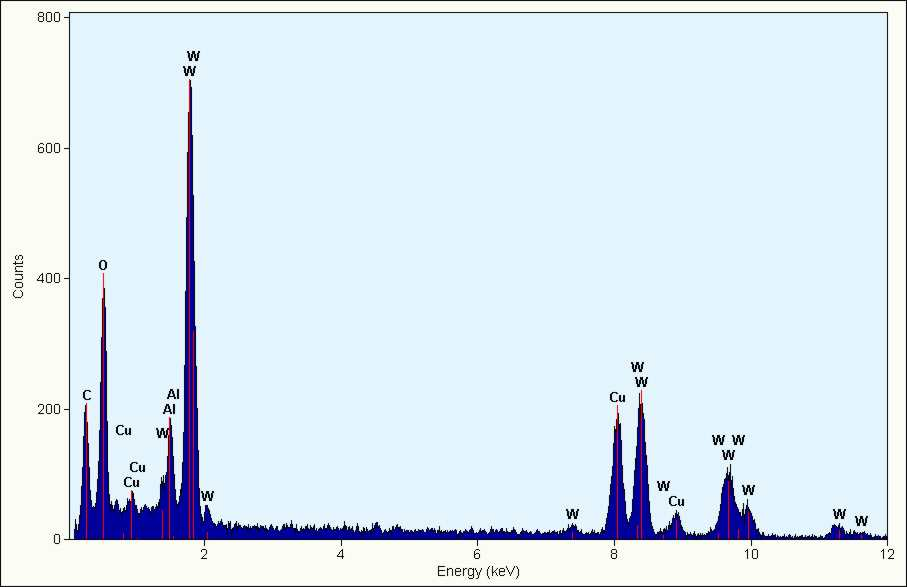
\includegraphics[width=\textwidth]{img/edx/beispiel_EDX.jpg}
    \caption*{ An example EDX spectrum for an aluminum tungsten oxide on a carbon foil supported on a copper grid. Adapted from \href{https://www.microscopy.ethz.ch/xray_spectrum.htm}{material prepared by Dr. Frank Krumeich.}}
\end{figure}

\pagebreak

Because the characteristic X-ray emission energies of any element are predictable and well-defined, the height and position of peaks they will produce on an EDX spectrum are also predictable and well-defined. For example:

\begin{itemize}
    \setlength\itemsep{-0.5em}
    \item Carbon will only ever produce a single peak at $\sim$ 277 eV.
    \item Oxygen will only ever produce a single peak at $\sim$ 525 eV.
    \item Silicon will only ever produce two characteristic X-rays: one at $\sim$ 1.74 keV and another at $\sim$ 1.84 keV. These peaks are too close to be distinguished by EDX detectors so only appear as one peak at $\sim$ 1.75 keV.
\end{itemize}

Heavier elements tend to produce more peaks at higher energies.

The characteristic X-ray energies that will be produced by each element can be found in various lookup tables, like \href{https://xdb.lbl.gov/Section1/Periodic_Table/X-ray_Elements.html}{this one from Lawrence Berkeley National Laboratory}. However, the most convenient and comprehensive resource for determining expected peaks is the software \href{https://www.cstl.nist.gov/div837/837.02/epq/dtsa2/index.html}{NIST DTSA-II}. DTSA-II also allows the user to simulate spectra and quantify elemental abundances from real spectra.

\subsection*{Background signal/continuum/bremsstrahlung and the Duane-Hunt limit}

Aside from the peaks produced by the characteristic X-rays of elements in a sample, an EDX spectrum will also feature a background signal (also called a ``continuum'') caused by \href{https://en.wikipedia.org/wiki/Bremsstrahlung}{bremsstrahlung (German for ``braking radiation'')}. These are X-rays emitted by the incident electrons being redirected by the atomic nuclei in the sample.

This background signal will take on a broad, hill-like distribution that tapers off at higher energies when using a low-energy electron beam (such as on an SEM instrument with an accelerating voltage on the order of 10 kV). When using a higher-energy electron beam (such as on a TEM instrument with an accelerating voltage on the order of 100 kV), this distribution will be much more spread out. Over the range of energies typically shown in EDX spectra (usually around 0 to 20 keV), the bremsstrahlung signal on a TEM EDX spectra will appear as low, constant-intensity background noise.

An EDX spectrum will only ever have a nonzero signal up to the energy of the incident electron beam. For example, if EDX is performed with an electron beam with an accelerating voltage of 10 kV, no elemental peaks or bremsstrahlung will be observed at energies higher than 10 keV. This is known as the \href{https://en.wikipedia.org/wiki/Duane%E2%80%93Hunt_law}{Duane-Hunt limit}.

\subsection*{Elements not detectable by EDX}

Hydrogen (atomic number 1) and helium (atomic number 2) do not produce characteristic X-rays and are thus not detectable by EDX. Lithium (atomic number 3) and beryllium (atomic number 4) produce characteristic X-rays at such a low energies ($\sim$ 54 and $\sim$ 108 keV, respectively) that most EDX detectors will fail to capture them.

\subsection*{Escape peaks}

Some elements will produce silicon "escape" peaks. These peaks occur with silicon-based detectors (used in the vast majority of EDX instruments) and will appear exactly one Si $K\alpha$ emission energy ($\sim$ 1.7 keV) below prominent peaks produced by an element. Some models of EDX instrument will remove escape peaks from the spectrum automatically.

\begin{figure}[h!tbp]
    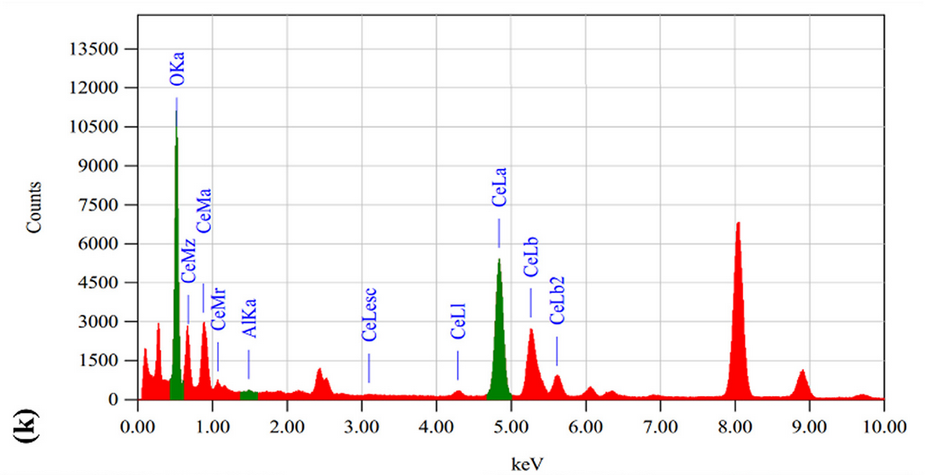
\includegraphics[width=\textwidth]{img/edx/shah_edx.png}
    \caption*{ An example EDX spectrum for a material containing cerium. A faint cerium escape peak is labeled at $\sim$ 3.1 keV. Adapted from Figure 3K of \href{https://doi.org/10.1016/j.ijhydene.2022.12.153}{Shah et al. (2023)}.}
\end{figure}

\subsection*{Zero strobe peak}

Many EDX detectors will insert an artificial peak centered at 0 eV. This peak, called the ``zero strobe'', ``zero strobe peak'' or ``strobe peak'', is used for instrument calibration is often removed before further analysis. If it is left included, it can give the appearance of detection of X-rays with negative energies. The appearance of a zero strobe peak in a published EDX spectrum is usually no cause for concern.

\begin{figure}[h!tbp]
    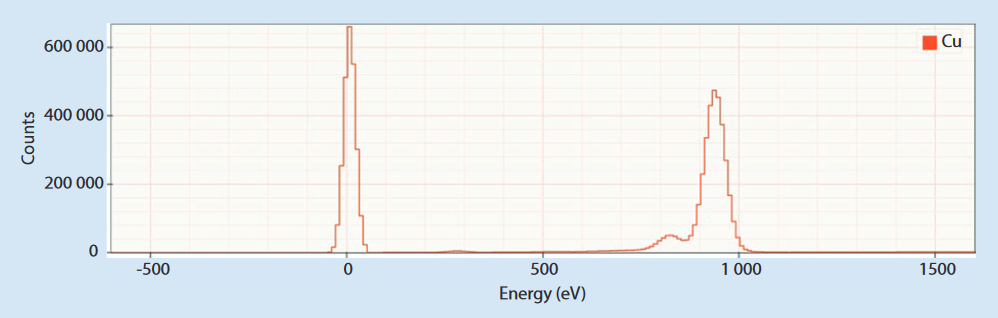
\includegraphics[width=\textwidth]{img/edx/zero_strobe_peak.png}
    \caption*{ An example EDX spectrum for elemental copper showing a zero strobe peak centered around 0 eV. Adapted from Figure 17.7 of \href{https://doi.org/10.1007/978-1-4939-6676-9}{Scanning Electron Microscopy and X-ray Microanalysis}.}
\end{figure}

\pagebreak

\subsection*{Sample preparation}

The optimal samples for EDX and the most suitable for quantitative analysis will have a flat, smooth, polished surface. Spectra from fibers, particles and rough surfaces can be collected, but only with a signficant reduction in accuracy.

If a sample is not conductive, a negative charge from the incident electron beam can build up on the sample surface, reducing the effective beam energy. This harms both EDX analysis and SEM visualization. To counteract this, samples are often coated with a conductive material. These materials will often appear as additional peaks in EDX spectra. Coatings are most commonly composed of carbon, gold, platinum, palladium, silver, iridium or chromium.

\subsection*{Mounting grids}

Samples are sometimes mounted to a metallic grid and/or a thin foil to facilitate handling (this is more common for EDX conducted with a TEM instrument). The materials used in these grids will often appear in EDX spectra. Grids and foils are most commonly composed of gold, copper, carbon or aluminum.

\subsection*{Example 1: Problematic EDX spectrum}

\href{https://doi.org/10.1016/j.ijhydene.2024.05.274}{Hussain et al. (2024)} claim to use EDX to characterize the elemental composition of an AgMnTe composite. However, the EDX spectrum they provide in Figure 2C has several issues:

\begin{enumerate}
    \setlength\itemsep{-0.5em}
    \item Tellurium has no peaks between 6 keV and 7 keV.
    \item Manganese has no peak at $\sim$ 6.2 keV.
    \item Manganese has no peak at $\sim$ 5 keV.
    \item The background signal is unusually tall and flat, which is not consistent with EDX performed on an SEM instrument.
\end{enumerate}

\begin{figure}[h!tbp]
    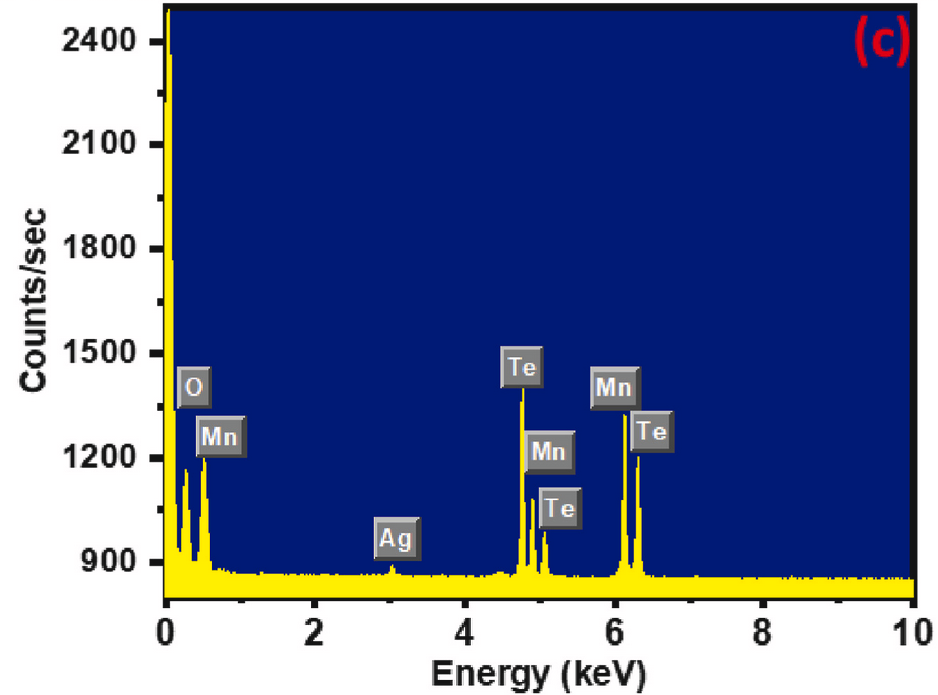
\includegraphics[width=\textwidth]{img/edx/hussain_edx.png}
    \caption*{ A problematic EDX spectrum with several nonsensical peak labels. Adapted from Figure 2C of \href{https://doi.org/10.1016/j.ijhydene.2024.05.274}{Hussain et al. (2024)}.}
\end{figure}

\pagebreak

\subsection*{Example 2: Problematic EDX spectrum}

\href{https://doi.org/10.1007/s10854-022-08265-y}{Alwadai et al. (2022)} claim to use EDX to characterize the elemental composition of polypyrrole, cobalt ferrite, and a poylpyrrole/cobal ferrite composite. However, the spectra they provide have numerous issues:

\begin{enumerate}
    \setlength\itemsep{-0.5em}
    \item Oxygen's sole peak should be at 524.9 eV, but appears in 3A at $\sim$ 0.9 keV.
    \item Oxygen has two peaks in 3B. Oxygen has one peak.
    \item Iron has no peaks between 1 and 4 keV. 3B shows two peaks for iron in this range.
    \item Iron has no peaks > 8 keV, unlike what is shown in 3B.
    \item Cobalt has no peak at $\sim$ 2 keV and no peak at $\sim$ 10 keV, unlike what is shown in 3B.
    \item In increasing order, the lowest energy peaks in 3C should be carbon, nitrogen, oxygen, iron. The order shown in 3C is nitrogen, oxygen, iron, carbon.
    \item Cobalt has no peaks at $\sim$ 5.9 keV. The nearest expected peak is an escape peak at $\sim$ 5.2 keV.
    \item Carbon does not have a peak at $\sim$ 7 keV.
    \item Oxygen does not have a peak at $\sim$ 8 keV.
    \item Hydrogen does not have any peaks, let alone one at $\sim$ 9 keV.
\end{enumerate}

\begin{figure}[h!tbp]
    \centering
    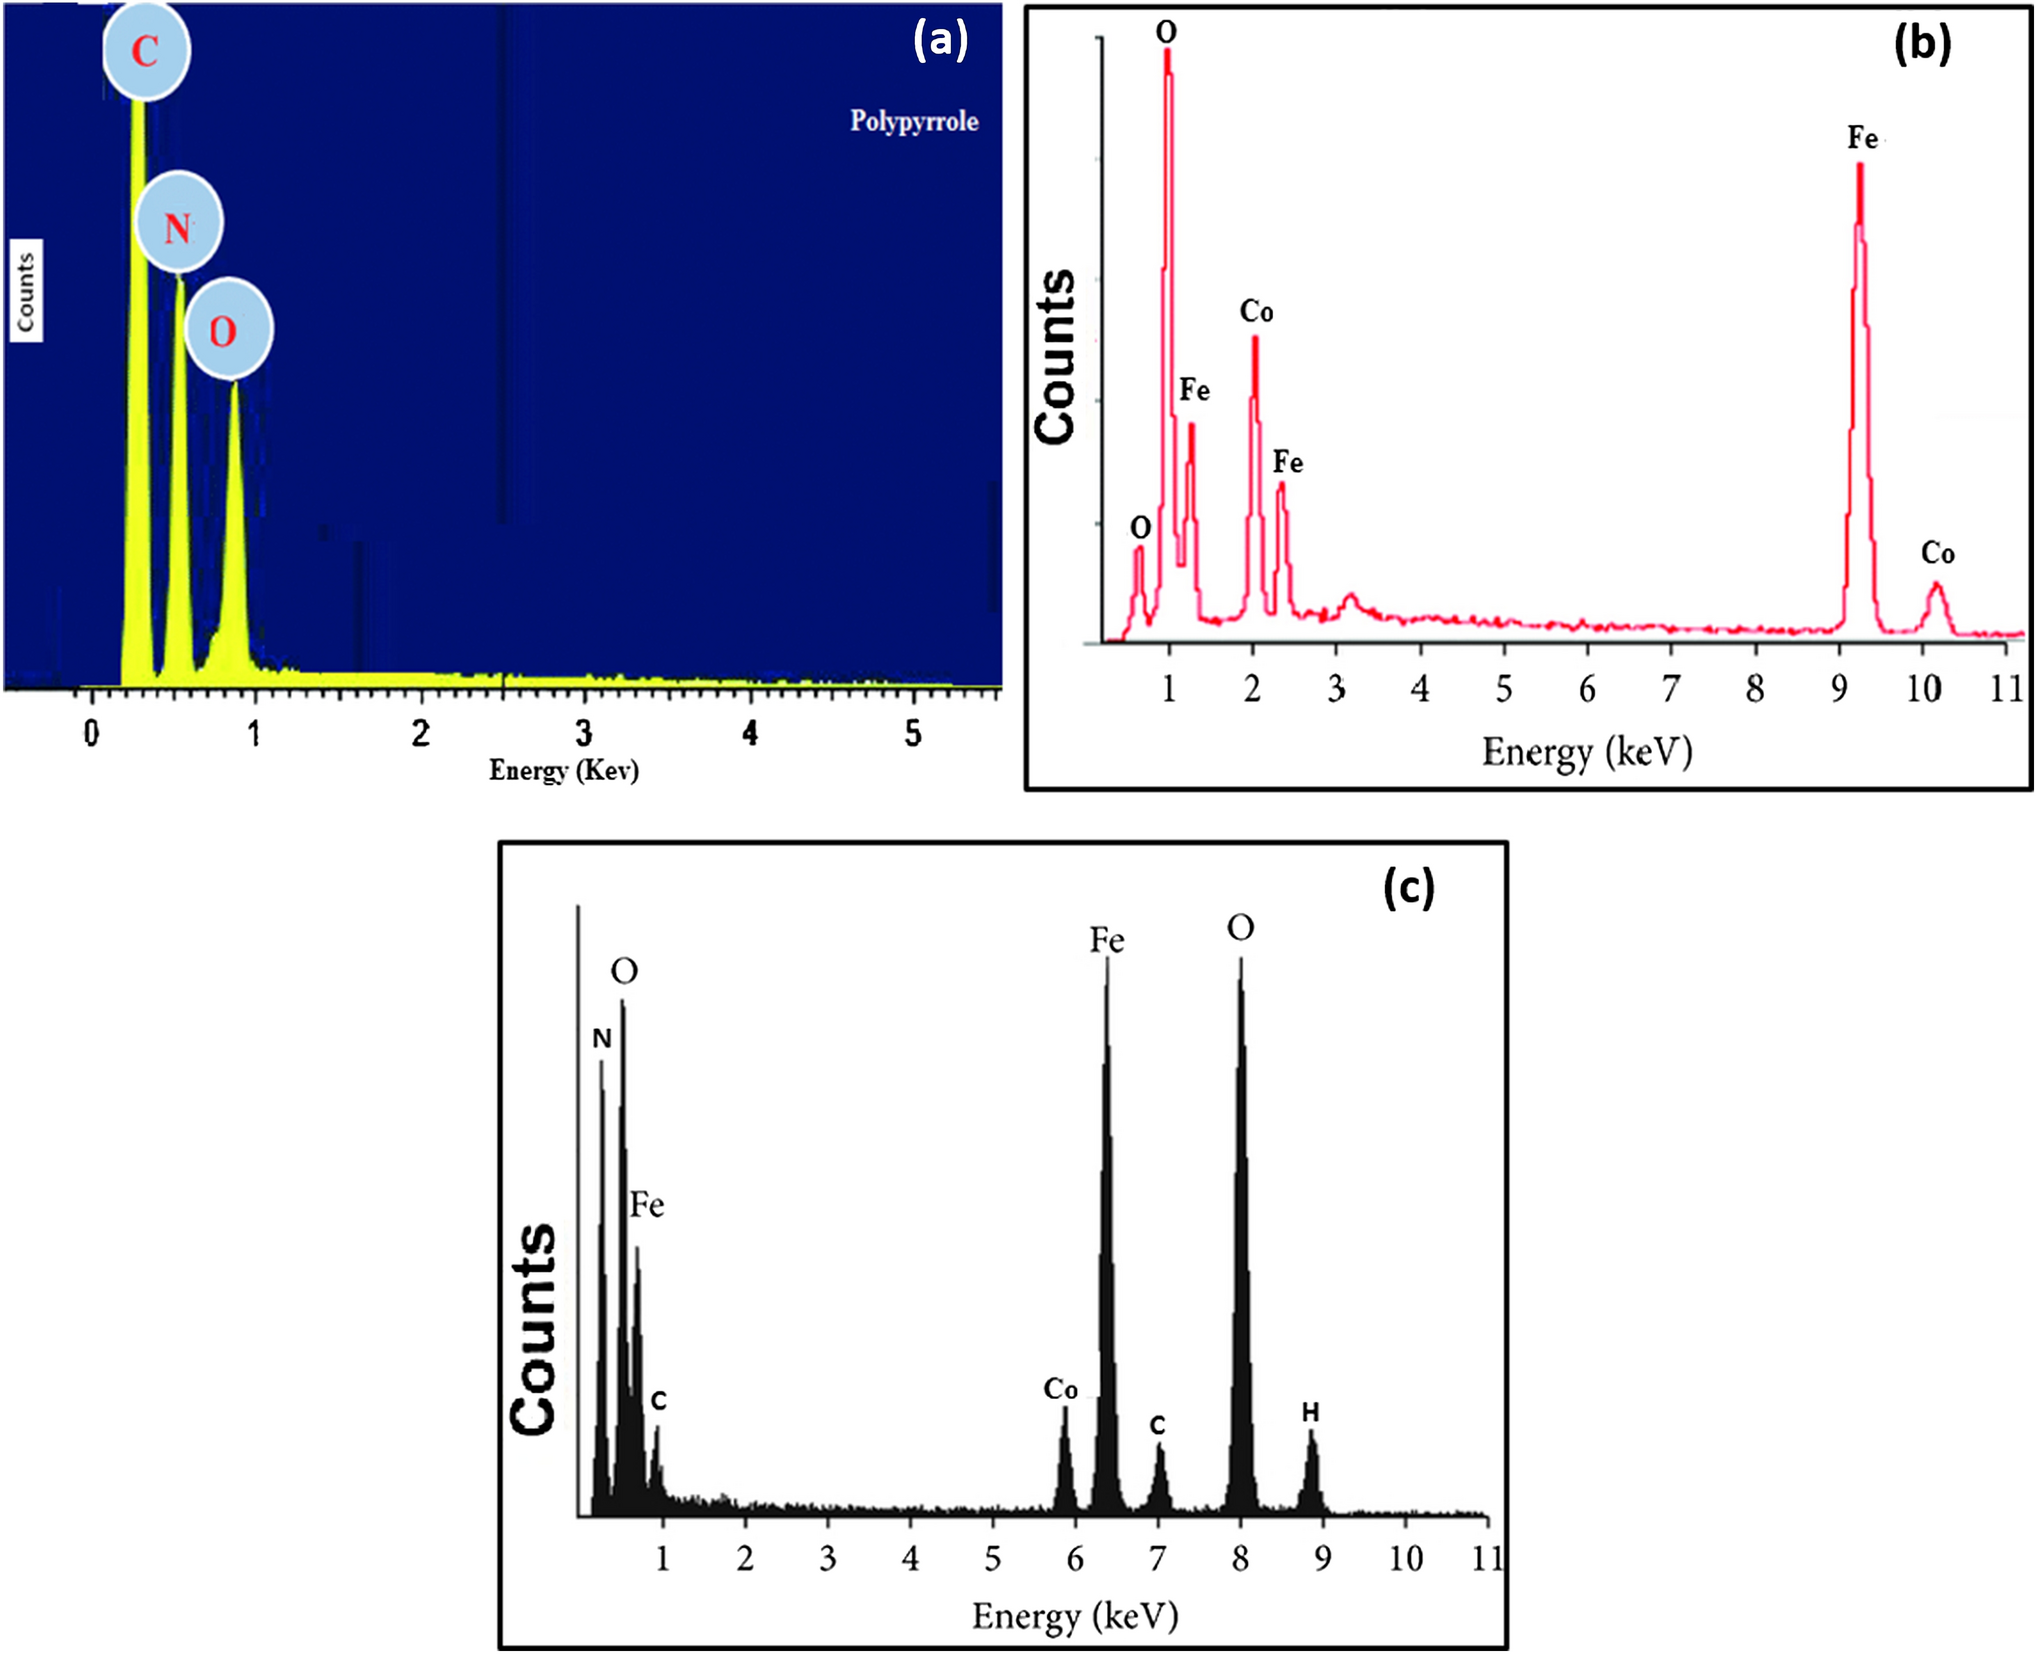
\includegraphics[width=0.8\textwidth]{img/edx/alwadai_edx.png}
    \caption*{Problematic EDX spectra with numerous issues. Adapted from Figure 3 of \href{https://doi.org/10.1007/s10854-022-08265-y}{Alwadai et al. (2022)}.}
\end{figure}

\subsection*{Additional resources}

\begin{itemize}
    \setlength\itemsep{-0.5em}
    \item \href{https://fy.chalmers.se/~f10mh/Halvarsson/EM_intro_course_files/EDX%20intro.pdf}{Lecture notes by Dr. Chris Boothroyd}
    \item \href{https://doi.org/10.1007/978-1-4939-6676-9}{\textit{Scanning Electron Microscopy and X-ray Microanalysis}}
    \item  \href{https://doi.org/10.6028/jres.107.051}{\textit{``Sample Preparation for Electron Probe
Microanalysis — Pushing the Limits"}}
    \item \href{https://doi.org/10.1007/s10853-014-8685-2}{"Performing elemental microanalysis with high accuracy and high precision by scanning electron microscopy/silicon drift detector energy-dispersive X-ray spectrometry (SEM/SDD-EDS)"}
    \item \href{https://www.cstl.nist.gov/div837/837.02/epq/dtsa2/index.html}{NIST DTSA-II}
\end{itemize}

% \setlength\itemsep{-0.5em}
% for bullet points and numbered lists.

\end{document}
\documentclass[letterpaper, 12pt]{article}

\usepackage{geometry}
 \geometry{
 letterpaper,
 total={170mm,257mm},
 left=20mm,
 top=20mm,
 bottom=20mm
 }
\usepackage{graphicx} % Required for inserting images
\usepackage{authblk}
\usepackage{amssymb}
\usepackage{lipsum}
\usepackage{float}
\usepackage{times}
\usepackage{amsmath}
\usepackage[format=plain,
            labelfont={bf,it},
            textfont=it]{caption}
\captionsetup{justification=raggedright,singlelinecheck=false}
\usepackage{ragged2e}
\usepackage{longtable}
\usepackage{comment}
\usepackage{setspace}
\usepackage{fancyhdr}
\usepackage{titlesec}
\usepackage[hyperindex,breaklinks]{hyperref}
\hypersetup{
    colorlinks=true,
    linkcolor=blue,
    filecolor=magenta,      
    urlcolor=blue,
    pdftitle={Overleaf Example},
    pdfpagemode=FullScreen,
    }
% \usepackage{background} % add COSIG logo to page
\usepackage[T1]{fontenc}
\usepackage{helvet}
\renewcommand{\familydefault}{\sfdefault}
\pagenumbering{gobble}
\usepackage[skip=10pt plus1pt, indent=40pt]{parskip}

\begin{comment}
\backgroundsetup{
   scale=1,
   angle=0,
   opacity=1,
   color=black,
   contents={\begin{tikzpicture}[remember picture, overlay]
      \node at ([xshift=3cm,yshift=1cm] current page.south west)
            {
\includegraphics[width = 5cm]{img/home/241017_final_logo_mockup.png}}; %<- change the name of image
     \end{tikzpicture}}
 }
\end{comment}

\titlespacing*{\section}
{0pt}{1.5ex plus 1ex minus .2ex}{1.3ex plus .2ex}

\renewcommand\Authfont{\fontsize{12}{14.4}\selectfont}
\renewcommand\Affilfont{\fontsize{9}{10.8}\itshape}

\begin{document}
\flushleft

\includegraphics[width=0.5\textwidth]{img/home/241017_final_logo_mockup.png}

\section*{Elemental composition}
\addcontentsline{toc}{section}{Elemental composition}
\textit{Last updated: 9 February 2025}

Different elements have different masses. For example, hydrogen has an atomic mass of 1.00784 u (atomic mass units), while oxygen has atomic mass of 15.999 u. Thus, although a molecule of water with molecular formula H$_2$O is composed of 66.6\% hydrogen and 33.3\% oxygen when counting atoms, it is 11.2\% hydrogen and 88.8\% oxygen by mass. These compositions are the water molecule's \textit{elemental atomic proportions} or \textit{atomic percentages} and the \textit{elemental mass proportions} or \textit{mass percentages} or \textit{weight percentages}, respectively.

Characterizing the elemental composition of a sample is an essential part of many chemistry and materials science studies. Elemental compositions are often determined by \href{https://en.wikipedia.org/wiki/Energy-dispersive_X-ray_spectroscopy}{energy dispersive x-ray spectroscopy (EDX/EDS/EDAX)} or \href{https://en.wikipedia.org/wiki/X-ray_photoelectron_spectroscopy}{X-ray photoelectron spectroscopy (XPS)}. You will often see these results provided in a table. In tables where both the atomic percentages and mass percentages for a compound/material are provided, they can be checked against one another. You can use \href{https://osf.io/gp4mf}{this spreadsheet} to convert between atomic percentages and mass percentages and vice-versa. These percentages can also be checked against what the authors claim the material is (see Example 3).

\subsection*{Isotopes}

Not all atoms of an element will have the same mass; different isotopes of an element can weigh different amounts. For example, the copper in the Earth's crust is about 69\% copper-63 (atomic mass 62.929 u) and about 31\% copper-65 (atomic mass 64.927 u). To account for the differing amounts of isotopes that will be found in a sample, chemists generally use a single \href{https://en.wikipedia.org/wiki/Standard_atomic_weight}{standard atomic weight} for each element. For copper, this value is 63.546 u (the weighted average of the atomic masses of the two copper isotopes commonly found in the Earth's crust).

Unless the authors of an article explicitly specify that they are quantifying the abundance of a specific isotope of an element, it is generally safe to use each element's standard atomic weight for fact-checking a composition table.

\subsection*{Should elemental composition percentages add up to 100\%?}

Techniques used for elemental composition quantification, like EDX, are associated with some analytical uncertainty. As a result, the elemental composition of a sample provided through EDX analysis may not add up to 100\%. The raw total of elemental composition percentages from EDX analysis is known as the ``analytical total'' (see the Discussion section of \href{https://doi.org/10.1007/s10853-024-10285-4}{Newbury and Ritchie, 2024}). 

Raw analytical totals can give an idea of the trustworthiness of an elemental analysis and should general fall between 98\% and 102\% (i.e., close to unity). Analytical totals far below 98\% can indicate that an element is present in a material but not included in the elemental composition analysis. 

Many authors, knowing that percentages \textit{should} add up to 100\%, will normalize their tables by this analytical total so that the reported percentages do add up to 100\%. This practice can conceal analytical errors and should generally be avoided.

In summary, elemental composition percentages that do not sum to 100\% but are otherwise close to 100\% are usually no cause for concern. However, elemental composition percentages that sum to a value far off from 100\% may be problematic.

\pagebreak

\subsection*{Example 1: No major issues with elemental composition table}

\href{https://doi.org/10.1080/10962247.2020.1813836}{Annamalai and Gurumurthy (2021)} report using EDX to quantify the elemental composition of electronic waste. In Table 4, the elemental weight percentages they report are entirely consistent with the elemental atomic percentages they report. There are no major issues with this analysis. However, the totals do add to up exactly 100\%, which suggests that this data has been normalized against the analytical total of elemental percentages. This practice can conceal analytical errors and is generally discouraged for EDX analysis.

\begin{figure}[h!tbp]
    \centering
    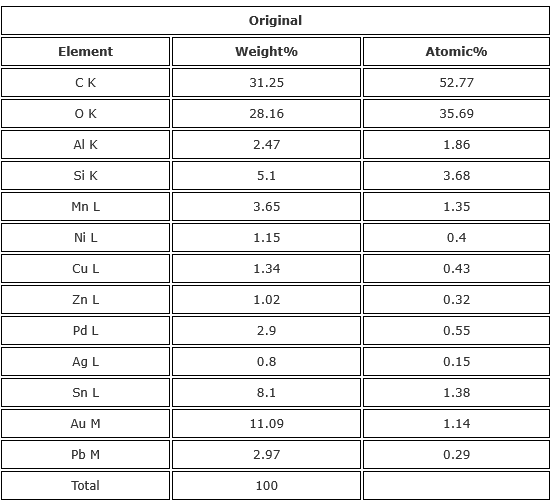
\includegraphics[width=0.8\textwidth]{img/elemental_composition/annamalai_gurumurthy_table_4.png}
    \caption*{An elemental composition table with no major detectable issues. Adapted from Table 4 of \href{https://doi.org/10.1080/10962247.2020.1813836}{Annamalai and Gurumurthy (2021)}.}
\end{figure}

\pagebreak

\subsection*{Example 2: Elemental atomic percentages do match elemental weight/mass percentages}

\href{https://doi.org/10.1016/j.photonics.2020.100889}{Salim et al. (2021)} report using EDX to quantify the elemental composition of amorphous cinnamon nanoparticles. However, in the inset table of Figure 2C, the claimed elemental atomic percentages are incompatible with the claimed elemental weight/mass percentages.

\begin{table}[h!tbp]
\begin{center}
\begin{tabular}{c|c|c|c}
Element & Claimed Wt\% 	& Claimed At\% 	& Calculated At\%\\
\hline
Cu 	& 44.2 	& 38.4 	& 16.3\\
C 	& 27.7 	& 23.9 	& 54.2\\
O 	& 13.5 	& 13.5 	& 19.8\\
S 	& 8.1 	& 8.2 	& 5.9\\
Ca 	& 4.7 	& 5.6 	& 2.8\\
Fe 	& 1.3 	& 4.8 	& 0.5\\
Na 	& 0.3 	& 3.4 	& 0.3\\
K 	& 0.2 	& 2.2 	& 0.1\\
\end{tabular}
\end{center}
\end{table}

\begin{figure}[h!tbp]
    \centering
    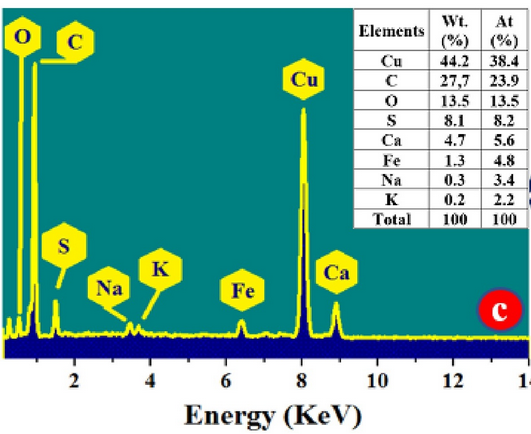
\includegraphics[width=0.8\textwidth]{img/elemental_composition/salim_table.png}
    \caption*{An elemental composition table where the claimed elemental atomic percentages are incompatible with the claimed elemental weight/mass percentages. Adapted from Figure 2C of \href{https://doi.org/10.1016/j.photonics.2020.100889}{Salim et al. (2021)}.}
\end{figure}

The EDX spectrum shown in this figure also has numerous issues. For more information, see the \href{https://osf.io/shfjy}{COSIG EDX guide}.

\subsection*{Example 3: Unexpected atomic percentages}

\href{https://doi.org/10.1371/journal.pone.0162891}{Mandizadeh et al. (2017)} report using EDX to confirm the elemental composition of SrCr$_x$Fe$_{12-x}$O$_{19}$ nanoceramics. However, for a sample that should have the molecular formula SrCr$_{0.5}$Fe$_{11.5}$O$_{19}$, they report the elemental atomic percentages as 3.95\% strontium, 64.27\% iron, 5.45\% chromium and 26.33\% oxygen. One would expect the oxygen proportion of their sample to be much closer to 19 oxygen atoms for every 32 atoms total ($\sim$ 59.4\%). The authors may have inadvertantly reported the elemental weight percentages as the elemental atomic percentages. Treating these percentages as the elemental weight percentages instead, we obtain a sample that is 1.5\% strontium, 39.1\% iron, 3.6\% chromium and 55.9\% oxygen by elemental atomic percentage, much closer to expectation.

\subsection*{Additional resources}

\begin{itemize}
    \setlength\itemsep{-0.5em}
    \item \href{https://doi.org/10.1007/s10853-024-10285-4}{``Testing the accuracy of low-beam-energy electron-excited X-ray microanalysis with energy-dispersive spectrometry'' (2024)}
    \item \href{https://doi.org/10.1017/S1431927619002964}{``Using the EDS Clues: Peak Fitting Residual Spectrum and Analytical Total'' (2019)}
    \item \href{https://doi.org/10.6028/jres.107.045}{``Limitations to Accuracy in Extracting Characteristic Line Intensities From X-Ray Spectra'' (2002)}
    \item \href{https://osf.io/shfjy}{COSIG: Energy-dispersive X-ray spectroscopy}
\end{itemize}

\end{document}
\documentclass[letterpaper, 12pt]{article}

\usepackage{geometry}
 \geometry{
 letterpaper,
 total={170mm,257mm},
 left=20mm,
 top=20mm,
 bottom=20mm
 }
\usepackage{graphicx} % Required for inserting images
\usepackage{authblk}
\usepackage{amssymb}
\usepackage{lipsum}
\usepackage{float}
\usepackage{times}
\usepackage{amsmath}
\usepackage[format=plain,
            labelfont={bf,it},
            textfont=it]{caption}
\captionsetup{justification=raggedright,singlelinecheck=false}
\usepackage{ragged2e}
\usepackage{longtable}
\usepackage{comment}
\usepackage{setspace}
\usepackage{fancyhdr}
\usepackage{titlesec}
\usepackage[hyperindex,breaklinks]{hyperref}
\hypersetup{
    colorlinks=true,
    linkcolor=blue,
    filecolor=magenta,      
    urlcolor=blue
    }
% \usepackage{background} % add COSIG logo to page
\usepackage[T1]{fontenc}
\usepackage{helvet}
\renewcommand{\familydefault}{\sfdefault}
\pagenumbering{gobble}
\usepackage[skip=10pt plus1pt, indent=40pt]{parskip}

\begin{comment}
\backgroundsetup{
   scale=1,
   angle=0,
   opacity=1,
   color=black,
   contents={\begin{tikzpicture}[remember picture, overlay]
      \node at ([xshift=3cm,yshift=1cm] current page.south west)
            {
\includegraphics[width = 5cm]{img/home/241017_final_logo_mockup.png}}; %<- change the name of image
     \end{tikzpicture}}
 }
\end{comment}

\titlespacing*{\section}
{0pt}{1.5ex plus 1ex minus .2ex}{1.3ex plus .2ex}

\renewcommand\Authfont{\fontsize{12}{14.4}\selectfont}
\renewcommand\Affilfont{\fontsize{9}{10.8}\itshape}
 
\begin{document}
\flushleft

\includegraphics[width=0.5\textwidth]{img/home/241017_final_logo_mockup.png}

\section*{Multiple hypothesis correction}
\addcontentsline{toc}{section}{Multiple hypothesis correction}
\textit{Last updated: 22 May 2025}

Scientific studies frequently involve \href{https://www.britannica.com/science/statistics/Hypothesis-testing}{statistical hypothesis testing}. For instance, scientists might test \href{https://doi.org/10.1038/s41598-023-49623-y}{whether birds from one region have longer beaks than birds from a different region}. For such a test, the null hypothesis ($H_0$) would probably be that there is no difference in beak length between the two populations and the alternative hypothesis ($H_a$) would be that their is a difference in beak length. By sampling individuals from both populations, measuring their beak lengths and comparing the beak lengths using a \href{https://en.wikipedia.org/wiki/Student%27s_t-test}{two-sample $t$-test}, these scientists can determine if there is sufficient statistical evidence to reject the null hypothesis. 

Usually, this is done by comparing a test's $p$ value to a signficance threshold $\alpha$. The $p$ value represents the probability of finding a statistical result as extreme as what was observed if the null hypothesis were indeed true (e.g., the probability of measuring the two different sampled means of beak length if the average beak lengths in the underlying populations were actually the same). Only rejecting the null hypothesis if $p < \alpha$ ensures that, for any given test, the probability of rejecting a true null hypothesis is less than $\alpha$. The most commonly-used $\alpha$ is $0.05$.

When testing a single hypothesis, you can usually rely on the unadjusted $p$ value of your statistical test to tell you whether or not you should reject your null hypothesis. However, many studies test many hypotheses at once. For instance, a study performing \href{https://www.ebi.ac.uk/training/online/courses/functional-genomics-ii-common-technologies-and-data-analysis-methods/rna-sequencing/performing-a-rna-seq-experiment/data-analysis/differential-gene-expression-analysis/#:~:text=Differential%20expression%20analysis%20means%20taking,expression%20levels%20between%20experimental%20groups}{differential expression analysis} on RNA sequencing data will test whether gene expression levels differ between a control group and a treatment group for thousands of genes at once. For experiments testing many hypotheses, it is useful to adjust these tests' $p$ values to prevent over-interpretation of results.

Consider a differential expression analysis experiment on 10,000 genes, none of which actually differ in their underlying expression levels for the two groups (i.e., the null hypothesis is true for all 10,000 genes). If changes in gene expression for each gene were determined using an unadjusted $p$ value below a threshold of $\alpha = 0.05$, then the null hypothesis would be rejected for around 500 genes, all of which would be false positives, also known as \href{https://en.wikipedia.org/wiki/Type_I_and_type_II_errors}{Type I errors}). To limit the number of false positives in an experiment like this, scientists will often use a multiple hypothesis correction procedure. This guide covers two of the most popular methods for multiple hypothesis correction, Bonferroni correction and Benjamini-Hochberg correction. Both methods will lower the threshold at which significance is called, decreasing the false positive rate (the rate at which correct null hypotheses are rejected) at the expense of increasing the false negative rate (the rate at which the null hypothesis is not rejected when the alternative hypothesis is true).

Experts are generally more concerned with mitigating false positives (i.e., false discoveries) than mitigating false negatives (i.e., ``missing something''), especially in certain fields (e.g., healthcare). A lack of multiple hypothesis correction leaves an experiment's results susceptible to over-interpretation.

\subsection*{Bonferroni correction}

Setting a significance threshold of $\alpha = 0.05$
ensures that, for a random individual test, the probability of rejecting a true null hypothesis is below 0.05. But what if we want to ensure that across all hypothesis testing performed, the probability of rejecting at least one true null hypothesis is below 0.05 (i.e., a 95\% chance of no false positives)?

This quantity (the probability of at least one false positive across all tests) is called the Family Wise Error Rate (FWER). There are a number of FWER-controlling procedures, but the most popular is \href{https://en.wikipedia.org/wiki/Bonferroni_correction}{Bonferroni correction}. Bonferroni correction controls the FWER to be $< \alpha$ by only rejecting the null hypothesis for test $i$ with $p$ value $p_i$ if
$$p_i \leq \frac{\alpha}{m}$$
where $m$ is number of tests performed (e.g., 10,000 genes). This can also be expressed as
$$p_i * m \leq \alpha.$$
A set of $p$ values can be Bonferroni-adjusted by multiplying them all by the number of tests performed and using the same significance threshold $\alpha$. Adjusted $p$ values (which we will call $p_i^{B}$) should be capped at 1.0.

Bonferroni correction is considered a very conservative procedure for multiple hypothesis correction. It is best to use in instances where there is a high cost for obtaining false positives.

\subsection*{Bejamini-Hochberg correction}

What if we wanted to ensure that across all positive calls (i.e., instances in which the null hypothesis is rejected), only a certain proportion are actually false positives?

This quantity (the number of false positive calls divided by the number of all positive calls) is the False Discovery Rate (FDR). The most popular FDR-controlling method is the \href{https://doi.org/10.1111/j.2517-6161.1995.tb02031.x}{Benjamini-Hochberg procedure}. Benjamini-Hochberg correction controls the FDR to be $< \alpha$ by only rejecting the null hypothesis for test $i$ with $p$ value $p_i$ if
$$p_i \leq \frac{r_i * \alpha}{m}$$
where $m$ is the number of tests and $r_i$ is the rank of $p$ value $p_i$ when all $p$ values are ranked from smallest (where $r = 1$) to largest (where $r = m$). This can also be expressed as
$$\frac{p_i * m}{r} \leq \alpha.$$
A set of $p$ values can be Benjamini-Hochberg-adjusted by multiplying each $p_i$ by the number of tests performed $m$, dividing each by their rank $r_i$, and using the same significance threshold $\alpha$. Adjusted $p$ values (which are often called $q$ values) should be capped at 1.0. If unadjusted $p$ values $p_i \leq p_j$, then it should also be the case that $q_i \leq q_j$. If $p_i \leq p_j$ but $q_i > q_j$, then $q_j$ should be set so that it is equal to $q_i$. In other words, $q$ values should increase \href{https://en.wikipedia.org/wiki/Monotonic_function}{monotonically} with their corresponding $p$ values.

The $q$ value of any test is the minimum FDR that can be attained across all tests if that value is called significant.

\subsection*{Example 1: Lack of multiple hypothesis correction, incorrect Benjamini-Hochberg calculation}

\href{https://doi.org/10.1073/pnas.2022857118}{Teruya et al. (2021)} report on performing whole-blood metabolomics to determine if there are any metabolites that are present at different abundance in the blood of dementia patients versus elderly controls. They perform hypothesis testing on 124 metabolites, finding 33 out of 124 to be significant at unadjusted $p < 0.05$. Using an unadjusted $p$ value to determine significance instead of using multiple hypothesis correction in this case likely means that the majority of what the authors call significantly-different ``dementia-linked markers'' are actually false positives.

If Benjamini-Hochberg correction was used and significance was called at $q < 0.05$, only 8 metabolites would be called as significant. The authors did perform Benjmanini-Hochberg multiple-hypothesis correction, but incorrectly. To compute $q$ values with this procedure, one would rank the $p$ values of the multiple tests from lowest (in this case, 1) to highest (in this case, 124), multiply each $p$ value by its rank, then divide each product by the number of tests performed (124). However, Table S2 shows that each product was instead divided by the number of tests called significant at $p < 0.05$ (33). Further, the calculation was only performed for those tests passing at this significance threshold.

This article has \href{https://doi.org/10.1073/pnas.2419538121}{since been corrected} to address this mistake. However, the authors still use unadjusted $p$ values to call for significantly different metabolites. This is especially problematic since there were only eight subjects per group, as \href{https://doi.org/10.1073/pnas.2118654119}{noted by others}.

\pagebreak

\begin{figure}[h!tbp]
    \centering
    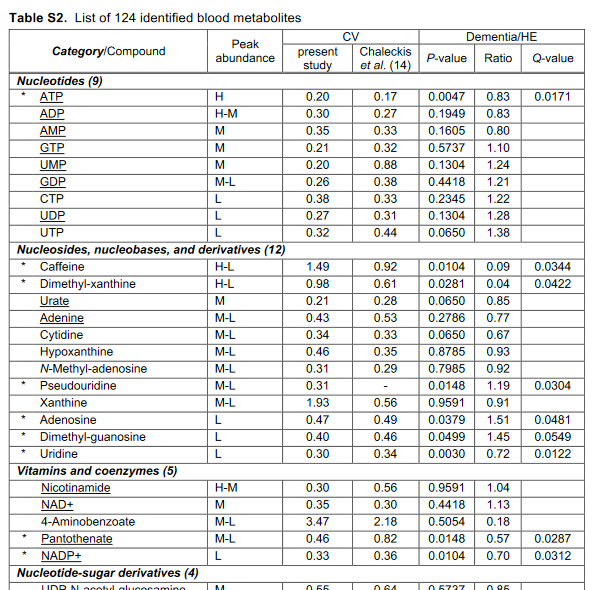
\includegraphics[width=0.8\textwidth]{img/multiple_hypothesis_correction/image-1715611965675.png}
    \caption*{The original Table S2 of \href{https://doi.org/10.1073/pnas.2022857118}{Teruya et al. (2021)}, which features incorrectly-calculated $q$ values.}
\end{figure}

\subsection*{Example 2: Lack of multiple hypothesis correction, inconsistency of $p$ values and $q$ values}

\href{https://doi.org/10.1096/fba.2020-00047}{Teruya et al. (2020)} report on performing metabolomics to determine if there are any metabolites that are present at different abundance in the urine of elderly individuals versus young individuals. They perform hypothesis testing on 99 metabolites, finding 55 out of 99 to be significantly different at unadjusted $p < 0.05$. Using an unadjusted $p$ value to determine significance instead of using multiple hypothesis correction in this case likely means that the majority of what the authors call significantly-different ``age-linked metabolites'' are actually false positives.

The authors do perform multiple hypothesis correciton with the Benjamini-Hochberg procedure, but appear not to use it for interpretation of their results. Instead, they state ``Q-values shown in Table S3 are consistent with p-values of 50 age-related compounds''.

However, the $q$ values shown in Table S3 do not increase monotonically with their corresponding $p$ values. There are some metabolites that depart wildly from the expected $q$ value, such as N-Acetyl-aspartate, with a $p$ value of 0.01675 and a $q$ value of 0.00045. It is not possible for any $q$ value to be less than its corresponding $p$ value.

\begin{figure}[h!tbp]
    \centering
    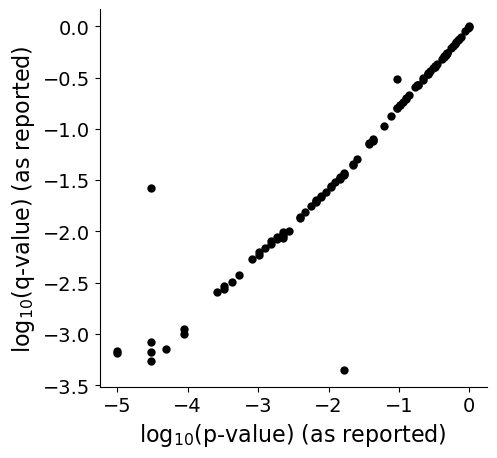
\includegraphics[width=0.8\textwidth]{img/multiple_hypothesis_correction/image-1715615096372.png}
    \caption*{A comparison of the $q$ values and $p$ values reported in Table S3 of \href{https://doi.org/10.1096/fba.2020-00047}{Teruya et al. (2020)}. Note that these $q$ values do not increase monotonically with their associated $p$ values, which should not be the case when using Benjamini-Hochberg correction.}
\end{figure}

\subsection*{Additional resources}

\begin{itemize}
    \setlength\itemsep{-0.5em}
     \item \href{https://www.graphpad.com/guides/prism/latest/statistics/stat_multiple_comparisons2.htm}{Prism 10 Statistics Guide: Multiple comparisons}
    \item \href{https://doi.org/10.1378/chest.11-0523}{``Correction for multiple testing: is there a resolution?'' (2011)}
    \item \href{https://doi.org/10.1038/nbt1209-1135}{``How does multiple testing correction work?'' (2010)}
    \item \href{https://doi.org/10.4045/tidsskr.21.0357}{``Adjustment of p-values for multiple hypotheses'' (2021, available in Norwegian and English)}
\end{itemize}

\end{document}
\documentclass[letterpaper, 12pt]{article}

\usepackage{geometry}
 \geometry{
 letterpaper,
 total={170mm,257mm},
 left=20mm,
 top=20mm,
 bottom=20mm
 }
\usepackage{graphicx} % Required for inserting images
\usepackage{authblk}
\usepackage{amssymb}
\usepackage{lipsum}
\usepackage{float}
\usepackage{times}
\usepackage{amsmath}
\usepackage[format=plain,
            labelfont={bf,it},
            textfont=it]{caption}
\captionsetup{justification=raggedright,singlelinecheck=false}
\usepackage{ragged2e}
\usepackage{longtable}
\usepackage{comment}
\usepackage{setspace}
\usepackage{fancyhdr}
\usepackage{titlesec}
\usepackage[hyperindex,breaklinks]{hyperref}
\hypersetup{
    colorlinks=true,
    linkcolor=blue,
    filecolor=magenta,      
    urlcolor=blue
    }
% \usepackage{background} % add COSIG logo to page
\usepackage[T1]{fontenc}
\usepackage{helvet}
\renewcommand{\familydefault}{\sfdefault}
\pagenumbering{gobble}
\usepackage[skip=10pt plus1pt, indent=40pt]{parskip}

\begin{comment}
\backgroundsetup{
   scale=1,
   angle=0,
   opacity=1,
   color=black,
   contents={\begin{tikzpicture}[remember picture, overlay]
      \node at ([xshift=3cm,yshift=1cm] current page.south west)
            {
\includegraphics[width = 5cm]{img/home/241017_final_logo_mockup.png}}; %<- change the name of image
     \end{tikzpicture}}
 }
\end{comment}

\titlespacing*{\section}
{0pt}{1.5ex plus 1ex minus .2ex}{1.3ex plus .2ex}

\renewcommand\Authfont{\fontsize{12}{14.4}\selectfont}
\renewcommand\Affilfont{\fontsize{9}{10.8}\itshape}
 
\begin{document}
\flushleft

\includegraphics[width=0.5\textwidth]{img/home/241017_final_logo_mockup.png}

\addcontentsline{toc}{part}{General guides}
\section*{PubPeer commenting best practices}
\addcontentsline{toc}{section}{PubPeer commenting best practices}
\textit{Last updated: 11 March 2025}

\href{https://pubpeer.com/}{PubPeer} is a post-publication peer review site where users can comment on any scientific publication. It is presently the foremost forum for post-publication peer review. To date, more than 200,000 scientific publications have been commented upon on PubPeer.

PuPubPeer comments can be posted anonymously, pseudonymously or under your name. Comments should be polite, neutral and should contribute meaningfully to scientific discussion. PubPeer employs a team of moderators that will edit or remove comments that do not meet these guidelines. For more information, read the \href{https://pubpeer.com/static/faq}{PubPeer FAQ} and \href{https://pubpeer.com/static/tos}{Terms of Service}.

This guide covers general tips on how to write a high quality, effective PubPeer comment.

\subsection*{Keep comments professional, direct, relevant and substantive}

PubPeer is a forum for facilitating scientific discourse. Comments should adopt a polite and neutral tone. Users should write with the goal of engaging readers and authors of a publication in discussion, not with the goal of airing their personal opinions or discussing matters that are not relevant to the publication at hand.

\subsubsection*{Examples of helpful comments}

\begin{quote}
    \textit{I see several issue with the analysis presenting in this article, which I elaborate upon below.}
\end{quote}

\begin{quote}
    \textit{We discussed this article in journal club and found the authors' investigation very thorough. Have the authors considered whether their method can be used for creating graphene-based catalysts?}
\end{quote}

\begin{quote}
\textit{Readers should become aware of a recent preprint by Jeannie Lee's group that used CLAP data to re-inforce the idea that PRC2 is an RNA binding protein. This preprint is entitled ``Re-analysis of CLAP data affirms PRC2 as an RNA binding protein'' and can be found at: \href{https://www.biorxiv.org/content/10.1101/2024.09.19.613009v1}{https://www.biorxiv.org/content/10.1101/2024.09.19.613009v1}}
\end{quote}

\subsubsection*{Examples of unhelpful comments}

\begin{quote}
    \textit{Great paper!}
\end{quote}

\begin{quote}
    \textit{This paper SUCKS! The authors should be ashamed of themselves.}
\end{quote}

\begin{quote}
    \textit{You are an imbecile extraordinaire. I will not dignify your comment with a response.}
\end{quote}

\begin{quote}
    \textit{Hahahahahaha}
\end{quote}

\begin{quote}
    \textit{This article reminds me of the time I caught the ferry over to Shelbyville. I needed a new heel for my shoe. So I decided to go to Morganville, which is what they called Shelbyville in those days. So I tied an onion to my belt, which was the style at the time. Now, to take the ferry cost a nickel...}
\end{quote}

\subsection*{Cite your sources and show your work}

As stated on the \href{https://pubpeer.com/static/faq#4}{PubPeer FAQ}, ``the most important rule for commenting is to base your statements on publicly verifiable information''. For effective comments, one should always clearly and thoroughly explain their reasoning and link to sources and supporting documents. Note that PubPeer comments can be styled with \href{https://pubpeer.com/static/markdown}{Markdown}, and thus allow for hyperlinking. For instance, a PubPeer comment written as
\begin{quote}
    \verb|Check out this [pre-print](doi.org/10.48550/arXiv.2107.06751)!|
\end{quote}

will appear on the site as

\begin{quote}
    \textit{Check out this \href{https://doi.org/10.48550/arXiv.2107.06751}{pre-print}!}
\end{quote}

\subsubsection*{Examples of helpful comments}

\begin{quote}
    \textit{The cell line \href{https://www.cellosaurus.org/CVCL_E307}{EC-9706} is contaminated by HeLa and is likely to be a poor model of esophageal cancer. See \href{https://faseb.onlinelibrary.wiley.com/doi/abs/10.1096/fj.14-266718}{``Genetic profiling reveals an alarming rate of cross-contamination among human cell lines used in China''}.}
\end{quote}

\begin{quote}
    \textit{The biological relevant molecular weight of Nrf2 is 95-110 kDa. However, in this paper they are studying an irrelevant protein at 68 kDa using Western immunoblotting. Please see Donna Zhang's article from 2013 for more information: \href{https://www.ncbi.nlm.nih.gov/pmc/articles/PMC3503463/}{https://www.ncbi.nlm.nih.gov/pmc/articles/PMC3503463/}}
\end{quote}

\begin{quote}
    \textit{
    Figure 7F: Authors source data match data points plotted in the Figure, but statistics appear different. “n = 3 Fire+/+ mice and 4 Fire $\Delta$/$\Delta$ mice. <0.3 $\mu$m, *P = 0.0417, two-way ANOVA with Sidak’s multiple comparisons test” Inputing the authors source data from the website: two-way ANOVA (genotype): F (1,25)=2.905. P=0.1007 (ns) two-way ANOVA (genotype/diameter interaction): F (1,25)=2.905. P=0.4333 (ns) Sidak’s multiple comparisons test (even though not valid as two-way ANOVA is ns): <0.3 (+/+ vs. $\Delta$/$\Delta$): t=2.422, DF=25, p=0.1099
}
\end{quote}

\subsubsection*{Examples of unhelpful comments}

\begin{quote}
    \textit{To achieve 16\% f>m, 39\% f=m, and 45\% m>f, the underlying normal distributions of f and m have a difference of d=0.63 [sd units]. [Moderator: you should show your work here.]}
\end{quote}

\begin{quote}
    \textit{Smith et al. covered a similar topic.}
\end{quote}

\subsection*{Include images and illustrate your observations}

As a part of ``showing your work'', it is helpful to readers to include pictures and illustrations in your comment. If you are leaving a comment about a particular figure, include that figure in the comment. If your observations about the figure are not immediately apparent, annotate that figure in a software like \href{https://www.microsoft.com/en-us/microsoft-365/powerpoint}{Microsoft PowerPoint}, \href{https://www.adobe.com/products/illustrator.html}{Adobe Illustrator}, \href{https://www.gimp.org/}{GIMP}, \href{https://inkscape.org/}{Inkscape} or \href{https://www.microsoft.com/en-us/windows/paint}{Microsoft Paint}. Note that externally-hosted images are backed up by PubPeer and will remain a part of the comment in perpetuity.

\subsubsection*{Examples of helpful comments}

\begin{quote}
    \textit{The SEM image shown in Figure 2B contains many apparent duplications. I have highlighted unexpectedly similar regions with colored boxes in the image below (brightness increased for ease of viewing).}
\end{quote}

\begin{figure}[h!tbp]
\centering
    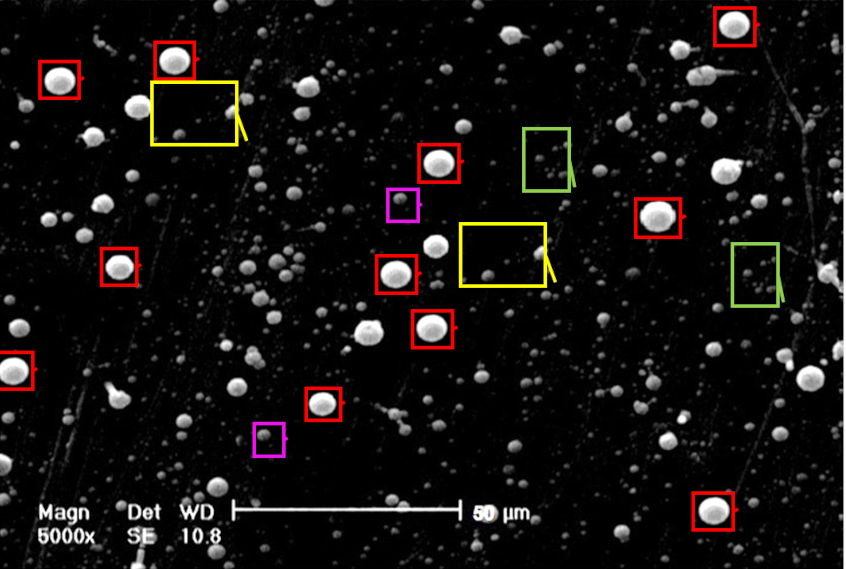
\includegraphics[width=0.8\textwidth]{img/pubpeer/pubpeer_dupes.PNG}
\end{figure}

\pagebreak
\begin{quote}
    \textit{Figure 6: Some of the images previously \href{https://pubpeer.com/publications/2E9CC5D00FDE41668A28B9622E64ED}{appeared elsewhere}. Identified by \href{https://imagetwin.ai}{Imagetwin.ai}.}
\end{quote}

\begin{figure}[h!tbp]
\centering
    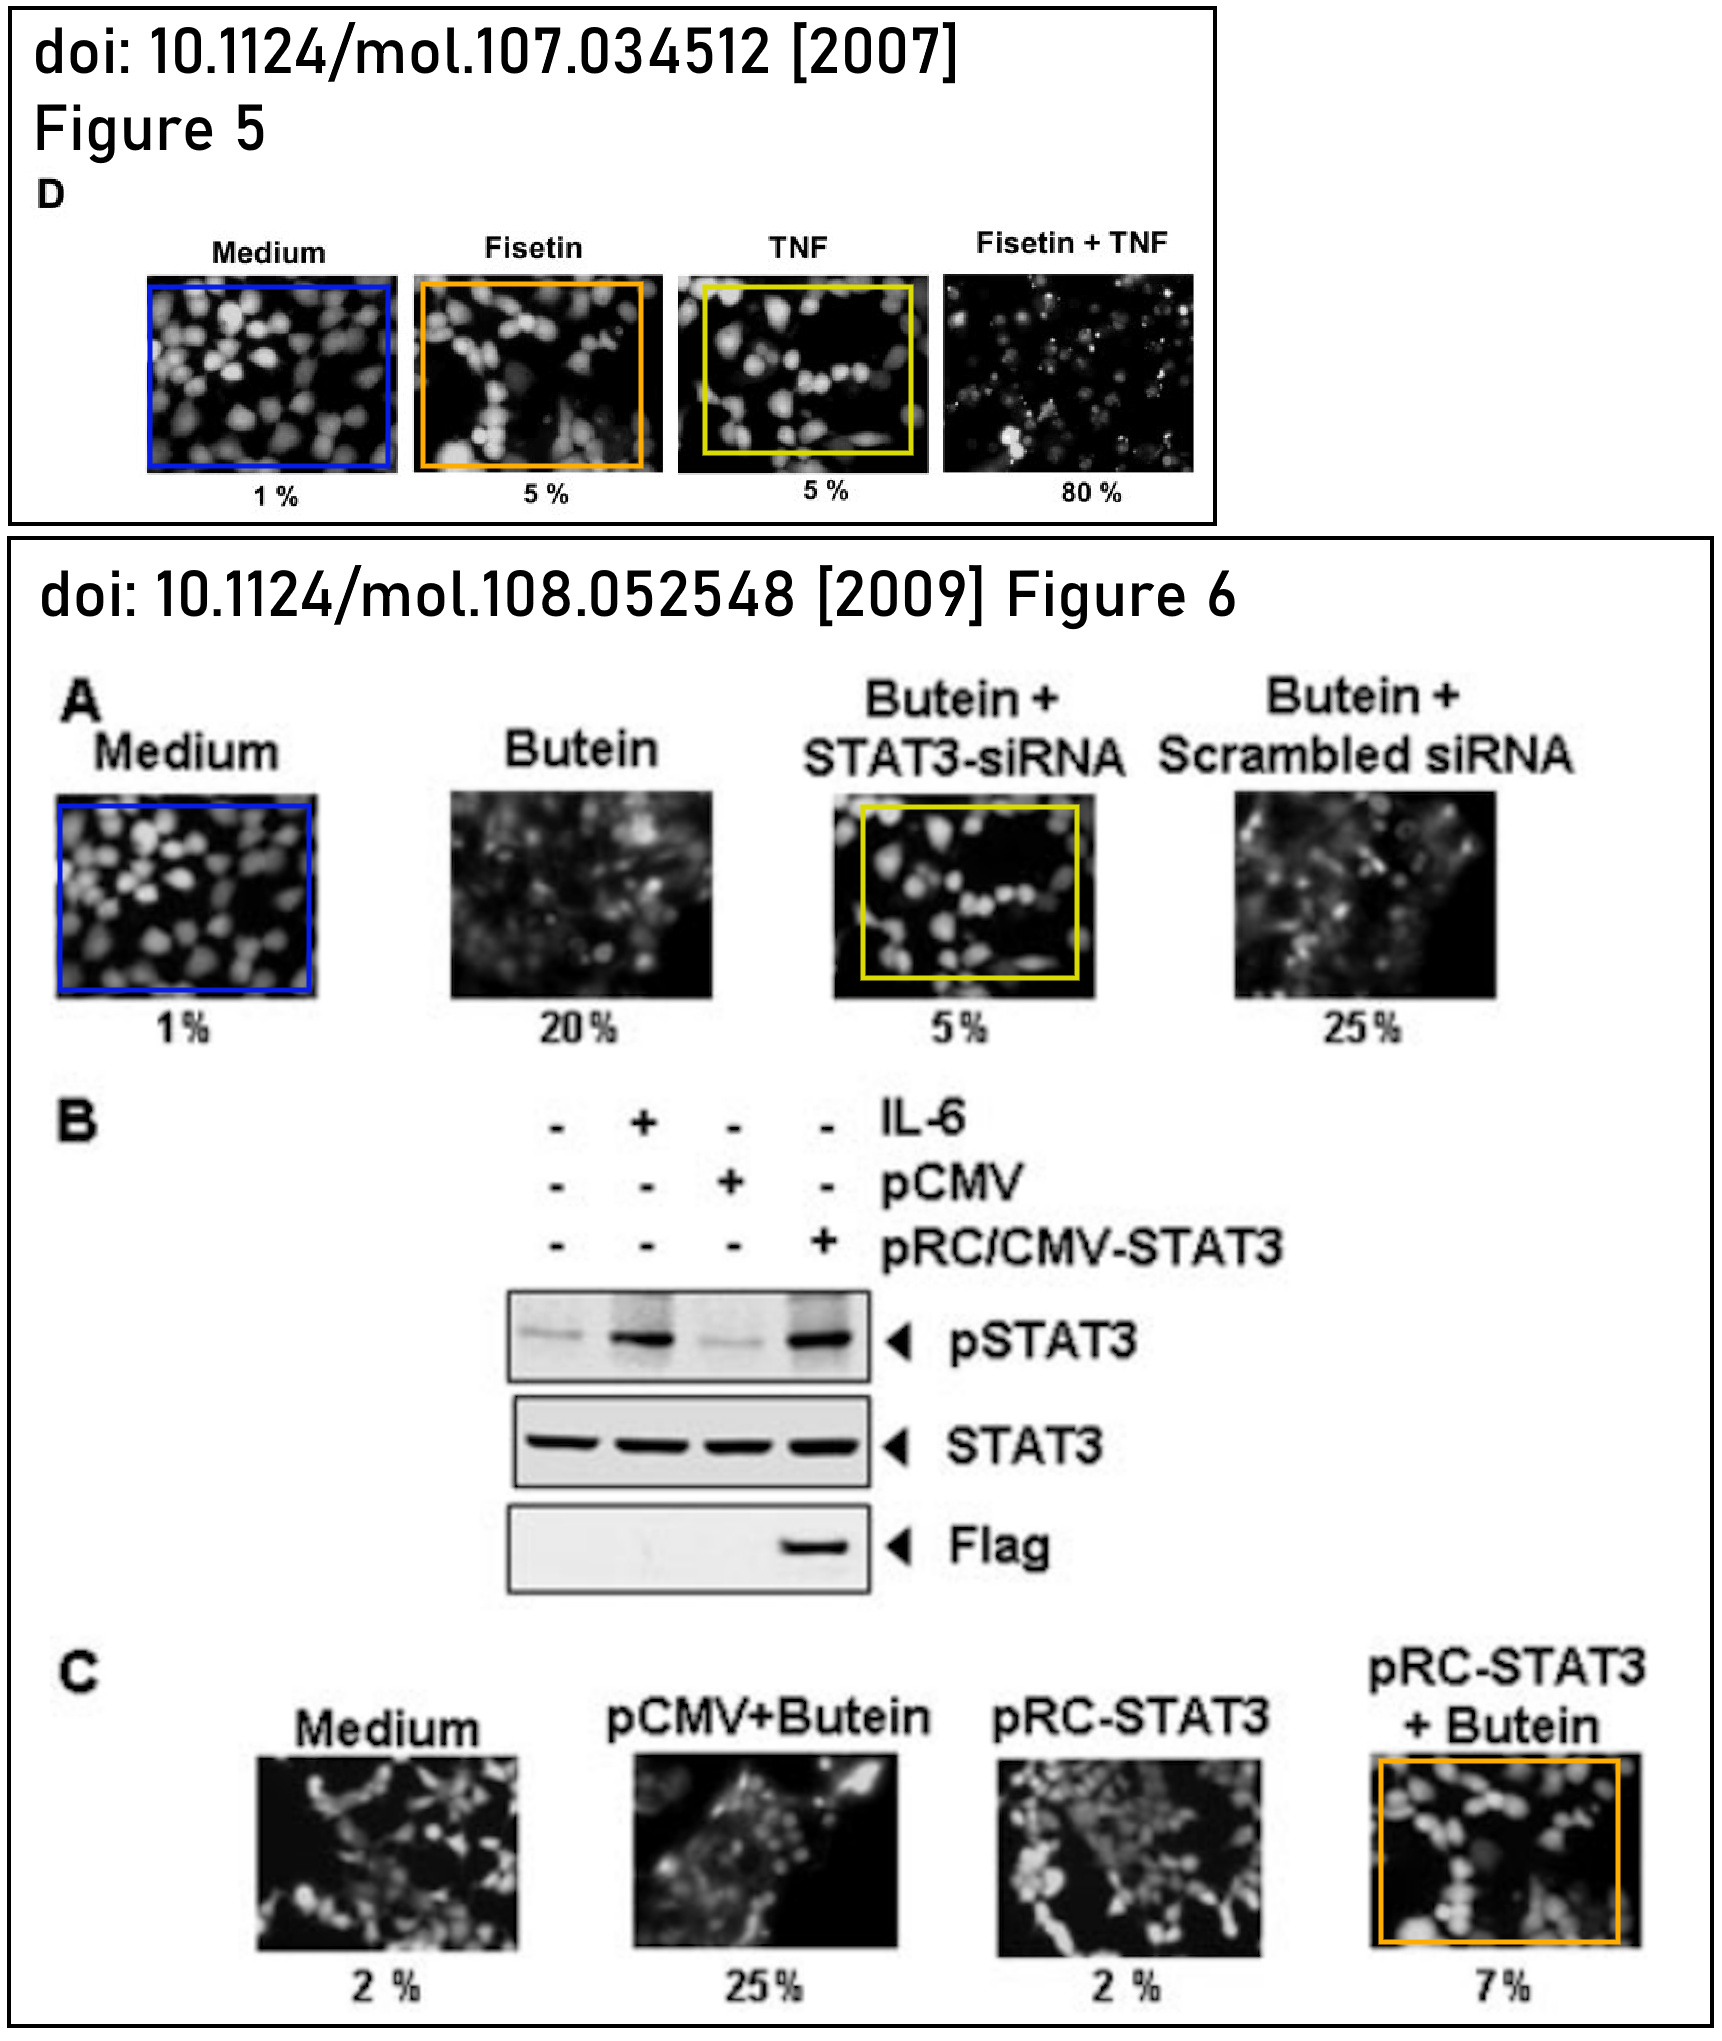
\includegraphics[width=0.5\textwidth]{img/pubpeer/image-1729709836291.png}
\end{figure}

\subsubsection*{Examples of unhelpful comments}

\begin{quote}
    \textit{The nanoparticles in Figure 8 look a bit wonky.}
\end{quote}

\begin{quote}
    \textit{Some of the lanes SDS-PAGE gel shown in Figure 4 look very similar to one another.}
\end{quote}

\subsection*{Do not speculate on researcher motivations}

Even when there is copious evidence that some fabrication, falsification or plagiarism occurred in a publication, it is not helpful to allege research misconduct. From the \href{https://pubpeer.com/static/faq#4}{PubPeer FAQ}:

\begin{quote}
    \textit{Allegations of misconduct are forbidden on PubPeer. They are anyway unnecessary. Your audience on the site is mostly composed of highly intelligent researchers and scientists. They are quite capable of drawing their own conclusions if the facts are clearly presented.}
\end{quote}

\begin{quote}
    \textit{You should also avoid personal comments about authors and speculation about researcher actions and motives. This is non-scientific, but also can pose legal problems.}
\end{quote}

Beyond this, it is often not possible to know exactly what took place in a publication's preparation and who was responsible for the improprieties observed in PubPeer comments.

\subsection*{Make specific, actionable requests from authors}

Authors are the best experts on their own publications and PubPeer has the option to provide author emails to loop them into a discussion. Questions about a publication can often be addressed directly by authors, so it is helpful to make clarifying requests where appropriate.

\begin{quote}
    \textit{Could the authors provide the original scanning electron microscope images shown in Figure 3?}
\end{quote}

\begin{quote}
    \textit{Could the authors provide the raw data for the EDX spectrum shown in Figure 4?}
\end{quote}

\begin{quote}
    \textit{Could the authors clarify how they estimated crystallite size?}
\end{quote}

\begin{quote}
    \textit{Could the authors clarify what ``enormous information'' means and why it was used instead of ``big data''?}
\end{quote}

\subsection*{Split multiple observations into multiple comments}

PubPeer comments can be referenced from other PubPeer comments on the same article by referring to the comment number preceded by ``\#''.

If you have many observations on different aspects of an article, consider splitting these observations into multiple comments so that other commenters can reference your specific observations one at a time.

\begin{figure}[h!tbp]
    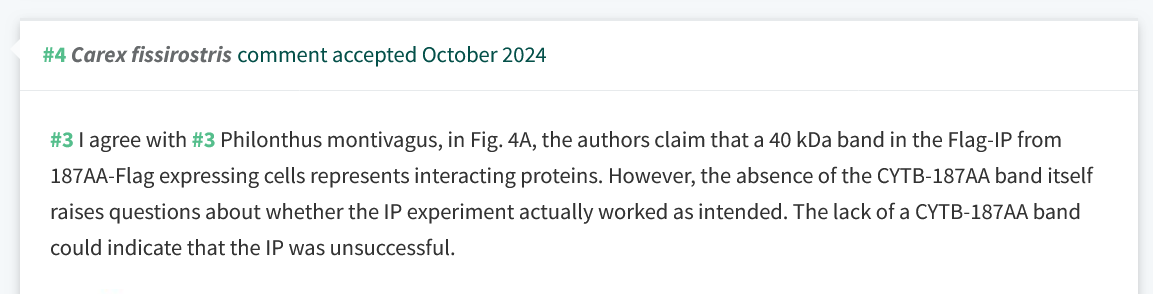
\includegraphics[width=\textwidth]{img/pubpeer/Screenshot 2024-10-23 at 16-36-04 PubPeer - A novel protein CYTB-187AA encoded by the mitochondrial gene.png}
    \caption*{This PubPeer comment refers back to a previous PubPeer comment using \#. The comment number for this comment can be found in the upper left corner of the comment box, to the left of the commenter's alias.}
\end{figure}
\end{document}
\documentclass[letterpaper, 12pt]{article}

\usepackage{geometry}
 \geometry{
 letterpaper,
 total={170mm,257mm},
 left=20mm,
 top=20mm,
 bottom=20mm
 }
\usepackage{graphicx} % Required for inserting images
\usepackage{authblk}
\usepackage{amssymb}
\usepackage{lipsum}
\usepackage{float}
\usepackage{times}
\usepackage{amsmath}
\usepackage[format=plain,
            labelfont={bf,it},
            textfont=it]{caption}
\captionsetup{justification=raggedright,singlelinecheck=false}
\usepackage{ragged2e}
\usepackage{longtable}
\usepackage{comment}
\usepackage{setspace}
\usepackage{fancyhdr}
\usepackage{titlesec}
\usepackage[hyperindex,breaklinks]{hyperref}
\hypersetup{
    colorlinks=true,
    linkcolor=blue,
    filecolor=magenta,      
    urlcolor=blue
    }
% \usepackage{background} % add COSIG logo to page
\usepackage[T1]{fontenc}
\usepackage{helvet}
\renewcommand{\familydefault}{\sfdefault}
\pagenumbering{gobble}
\usepackage[skip=10pt plus1pt, indent=40pt]{parskip}

\begin{comment}
\backgroundsetup{
   scale=1,
   angle=0,
   opacity=1,
   color=black,
   contents={\begin{tikzpicture}[remember picture, overlay]
      \node at ([xshift=3cm,yshift=1cm] current page.south west)
            {
\includegraphics[width = 5cm]{img/home/241017_final_logo_mockup.png}}; %<- change the name of image
     \end{tikzpicture}}
 }
\end{comment}

\titlespacing*{\section}
{0pt}{1.5ex plus 1ex minus .2ex}{1.3ex plus .2ex}

\renewcommand\Authfont{\fontsize{12}{14.4}\selectfont}
\renewcommand\Affilfont{\fontsize{9}{10.8}\itshape}
 
\begin{document}
\flushleft

\includegraphics[width=0.5\textwidth]{img/home/241017_final_logo_mockup.png}

\section*{Reporting publication integrity issues to publishers}
\addcontentsline{toc}{section}{Reporting publication integrity issues to publishers}
\textit{Last updated: 13 May 2025}

\subsection*{Integrity/ethics teams at publishers}

Most of the large scientific publishers have whole departments for publication ethics and publication integrity. These departments investigate incoming reports of possible errors and will advise editors and editors-in-chief on how to correct the scientific record. Usually these departments will follow the guidelines set by the \href{https://publicationethics.org/}{Committee on Publication Ethics (COPE)}, which generally consists of reviewing the evidence, contacting the journal and authors and coming to some sort of closure.

\subsection*{How to report issues to publishers}

The best way to reach these teams is by email. You can send this email both to the publisher's integrity team as well as to the journal's editors-in-chief. Some journals will have editorial board members that specifically handle ethics concerns or certain topics (e.g., disciplinary fields or specific methodologies).

Just as described in the guide for \href{https://osf.io/sghaq}{PubPeer commenting best practices}, you should be clear and neutral when describing potential publication integrity issues to these teams. Always include the \href{https://www.doi.org/}{DOI} (or other permanent identifier, such as PubMed ID) of the article(s) in question and report in a neutral way about the issue(s). Including a link to PubPeer where the issues are discussed in greater depth or an including an image to illustrate an issue may be useful.

Always be respectful when you contact publishers' integrity teams. Do not project frustrations or anger onto the members of these teams. Feel free to ask for a confirmation of receipt at the end of your email in order to make sure that the recipient has received all the relevant information.

\subsection*{Example of a helpful email to a publisher}

\begin{quote}
\textit{To whom it may concern,}\\
\indent\\
\textit{We have detected duplicated images in figures of articles published in [journal].}\\
\indent\\
\textit{We found an overlap between figure 1, panel A of Article 1 [DOI] and Figure 5, panel B of Article 2 [DOI]. We also found an overlap between Figure 3, panel C of Article 1 [DOI] and Figure 1, panel E of Article 3 [DOI].}\\
\indent\\
\textit{All of our findings have also been made publicly available on PubPeer:}\\
\indent\\
\textit{Article 1: [PubPeer link]\\
Article 2: [PubPeer link]\\
Article 3: [PubPeer link]\\}
\indent\\
\textit{Feel free to contact us with your questions. We’re happy to clarify any issues you might have. Could all of the recipients send us a confirmation of receipt of this email and let us know what the timeframe will be for assessing these issues?}\\
\indent
\textit{Best,}\\
\indent\\
\textit{[Name/pseudonym]}
\end{quote}

\subsection*{What happens next?}

You should be very patient after reporting an issue; investigations often take months if not years to resolve, even for blatant issues that seem to warrant immediate action. A publisher's integrity team may take one of several actions after being contacted regarding a publication integrity or ethics issue:

\begin{itemize}
    \setlength\itemsep{-0.5em}
    \item When an investigation finds that the conclusions of the research are not affected, the authors will be given the chance to clarify or correct their article post-publication. This will be often done in the form of a \textit{correction}, which should detail what the initial problem was and how the problem was resolved.
    \item When an investigation finds that conclusions of the research are affected or the work cannot be trusted, the article will usually be \textit{retracted}. A retraction note will be published, detailing why the problem was too substantial to correct.
    \item When it is unclear whether the conclusions are affected by the reported issue, an \textit{expression of concern} might be issued. This is a way for publishers to show that readers should exercise increased caution when interpreting the results of the published article.
    \item Nothing happens. Research integrity teams handle many cases and may drop a case with or without notifying the party that raised the issue.
\end{itemize}

When reporting an issue, you may ask to be notified when an investigation is resolved or an editorial notice is applied to an article. COPE \href{https://doi.org/10.24318/cope.2019.2.25}{recommends} that editors inform the person that originally raised concerns when the an outcome is reached, but many publishers fail to adhere to this guidance.

\pagebreak
\subsection*{Contact information for integrity/ethics teams at major publishers}

\begin{itemize}
    \setlength\itemsep{-0.5em}
    \item American Chemical Society (ACS): Each journal usually has contact information for a managing editor, usually at managing.editor@<journal-url>.org
    \item American Society for Microbiology: ethics.journals@asmusa.org
    \item British Medical Journal (BMJ): publication.ethics@bmj.com
    \item Elsevier (Elsevier, Cell Press): ethicsexpert@elsevier.com
    \item Frontiers: research.integrity@frontiersin.org
    \item IEEE: pub-ethics@ieee.org
    \item Karger: publication.ethics@karger.com
    \item MDPI: publication.ethics@mdpi.com
    \item Oxford University Press: journals.ethics@oup.com
    \item PLOS: pub-ethics@plos.org
    \item Rockefeller University Press (Journal of Cell Biology, Life Science Alliance): integrity@rupress.org
    \item Sage (Sage, Mary-Ann Liebert): publication\_ethics@sagepub.com
    \item Springer Nature (Springer, Nature, BMC): ethics.reporting@springernature.com
    \item Taylor \& Francis (Taylor \& Francis, Dove Medical Press, CRC Press, Routledge): ethics@tandf.co.uk
    \item Wiley (Wiley, Hindawi, FEBS Press): researchintegrity@wiley.com
\end{itemize}

\subsection*{Additional resources}

\begin{itemize}
    \setlength\itemsep{-0.5em}
    \item \href{https://doi.org/10.3145/epi.2023.ene.18}{``How do journals deal with problematic articles. Editorial response of journals to articles commented in PubPeer'' (2023)}
\end{itemize}

\end{document}
\documentclass[letterpaper, 12pt]{article}

\usepackage{geometry}
 \geometry{
 letterpaper,
 total={170mm,257mm},
 left=20mm,
 top=20mm,
 bottom=20mm
 }
\usepackage{graphicx} % Required for inserting images
\usepackage{authblk}
\usepackage{amssymb}
\usepackage{lipsum}
\usepackage{float}
\usepackage{times}
\usepackage{amsmath}
\usepackage[format=plain,
            labelfont={bf,it},
            textfont=it]{caption}
\captionsetup{justification=raggedright,singlelinecheck=false}
\usepackage{ragged2e}
\usepackage{longtable}
\usepackage{comment}
\usepackage{setspace}
\usepackage{fancyhdr}
\usepackage{titlesec}
\usepackage[hyperindex,breaklinks]{hyperref}
\hypersetup{
    colorlinks=true,
    linkcolor=blue,
    filecolor=magenta,      
    urlcolor=blue,
    pdftitle={Overleaf Example},
    pdfpagemode=FullScreen,
    }
% \usepackage{background} % add COSIG logo to page
\usepackage[T1]{fontenc}
\usepackage{helvet}
\renewcommand{\familydefault}{\sfdefault}
\pagenumbering{gobble}
\usepackage[skip=10pt plus1pt, indent=40pt]{parskip}

\begin{comment}
\backgroundsetup{
   scale=1,
   angle=0,
   opacity=1,
   color=black,
   contents={\begin{tikzpicture}[remember picture, overlay]
      \node at ([xshift=3cm,yshift=1cm] current page.south west)
            {
\includegraphics[width = 5cm]{img/home/241017_final_logo_mockup.png}}; %<- change the name of image
     \end{tikzpicture}}
 }
\end{comment}

\titlespacing*{\section}
{0pt}{1.5ex plus 1ex minus .2ex}{1.3ex plus .2ex}

\renewcommand\Authfont{\fontsize{12}{14.4}\selectfont}
\renewcommand\Affilfont{\fontsize{9}{10.8}\itshape}
 
\begin{document}
\flushleft

\includegraphics[width=0.5\textwidth]{img/home/241017_final_logo_mockup.png}

\section*{Standard deviation versus standard error}
\addcontentsline{toc}{section}{Standard deviation versus standard error}
\textit{Last updated: 6 February 2025}

\subsection*{Standard deviation}

\href{https://en.wikipedia.org/wiki/Standard_deviation}{Standard deviation (SD)} is a statistical measure that describes the variability of numerical observations of a variable around the mean of these observations.

When an entire population is measured, the population standard deviation is calculated $\sigma$ is calculated as 

$$
\sigma = \sqrt{\frac{\sum(x_i - \bar{x})^2}{N}}
$$

where $x_i$ is the value of each observation, $\bar{x}$ is the mean of each observation ($\bar{x} = \sum x_i / N$) and $N$ is the number of observations (i.e., the sample size). A lower standard deviation indicates that the data is more closely clustered around its mean, whereas a higher standard deviation indicates that the data is more spread out from its mean.

Note that standard deviation is calculated differently depending on whether you are measuring standard deviation for a population versus just a sample from that population. When only a sample is taken from a population, the sample standard deviation $s$ is calculated as 

$$
s = \sqrt{\frac{\sum(x_i - \bar{x})^2}{N-1}}.
$$

See \href{https://digitalcommons.unl.edu/cgi/viewcontent.cgi?article=1008&context=imseteach}{this explanation by Dr. Paul Savory} for why this correction is made. Most research does not survey a whole population, and thus ``standard deviation" usually denotes sample standard deviation $s$ and not population standard deviation $\sigma$.

Imagine that we took a sample of ten individuals and measured their height in centimeters, obtaining ten observations: 176, 171, 159, 168, 185, 193, 174, 171, 168 and 189. The mean of this sample would be 175.4 and the sample standard deviation would be approximately 10.6.

\subsection*{Standard error}

\href{https://en.wikipedia.org/wiki/Standard_error}{Standard error (SE)} is a measure of the variability of an estimate. For instance, for the previous scenario, a different sample of ten individuals would likely yield a slightly different mean height. The standard error $SE$ is calculated as

$$
SE = \frac{s}{\sqrt{N}}.
$$

Note that as sample size $N$ increases, the standard error decreases. For instance, the mean heights calculated from two different samples of 100 from the same population would likely be closer together than the mean heights calculated from two different samples of only 10. This is why studies with a larger sample size are generally considered more rigorous; their estimates will be more precise. For the previously-listed sample of heights, the standard error of the mean (SEM) would be $10.6/\sqrt{10} \approx 3.3$.

\subsection*{Reporting of standard deviation versus standard error}

When reading a scientific publication, one should take note of whether the authors are reporting variability in their data as standard deviation or standard error. Misidentifying which measure is being reported can give the reader an unrealistic picture of the variability in data and the uncertainty of estimates. There is some evidence that using one measure or the other graphically can lead to this same misinterpretation, even when the reader is aware of which measure is being used (see \href{https://doi.org/10.1073/pnas.2302491120}{Zhang et al., 2023}).

\begin{figure}[h!tbp]
    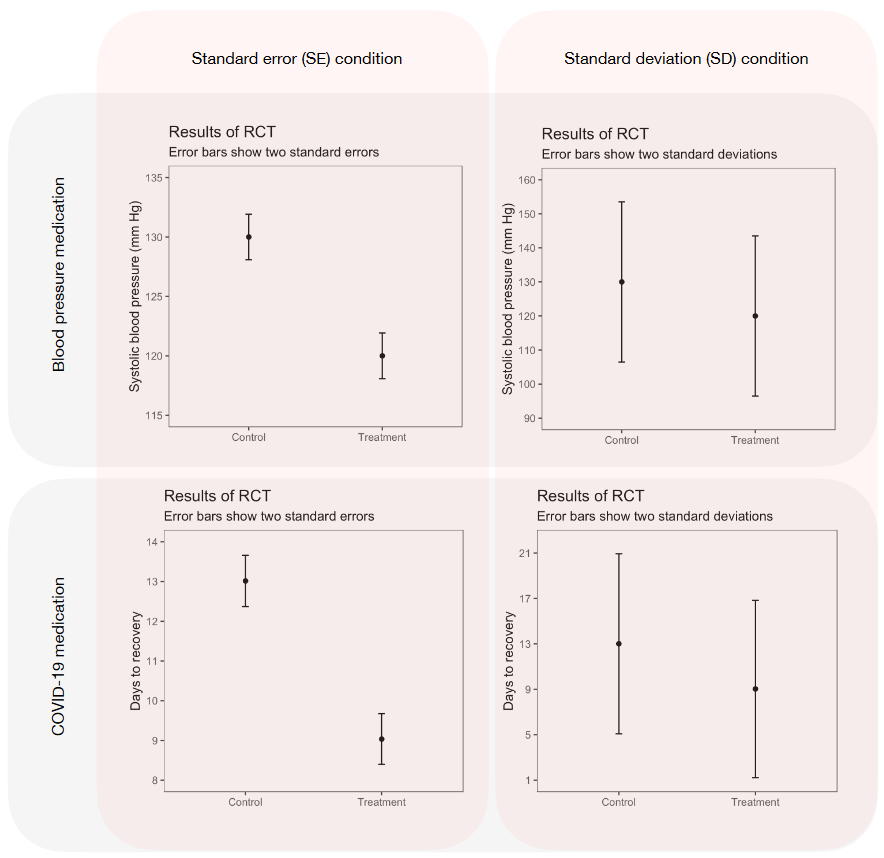
\includegraphics[width=\textwidth]{img/sd_vs_se/zhang_se_vs_sd.png}
    \caption*{Within each row, both charts demonstrate the same hypothetical data from a randomized controlled trial (for blood pressure medication, top row, or COVID-19 medication, bottom row). However, the left charts use error bars to display standard error of the mean and the right charts use error bars to display standard deviation. Adapted from Figure S1 of \href{https://doi.org/10.1073/pnas.2302491120}{Zhang et al. ( 2023)}.}
\end{figure}

\pagebreak

\subsection*{Incorporating variability into a meta-analysis}

A \href{https://en.wikipedia.org/wiki/Meta-analysis}{meta-analysis} is a study that synthesizes the results of independent studies on the same topic to obtain more precise estimates. For instance, one might perform a meta-analysis of randomized controlled trials that all tested the same drug to more precisely determine how effective the drug is at preventing intensive care unit admission or mortality due to COVID-19.

Because larger studies give more precise estimates, they are usually given more weight in meta-analyses so that their findings contribute more to the combined outcome estimate. The most common method for weighting studies for meta-analysis is \href{https://training.cochrane.org/handbook/current/chapter-10#section-10-3}{inverse variance weighting}. With inverse variance weighting, each study is weighted by

$$
\frac{1}{SE^2}
$$

where $SE$ is the standard error of that study's estimate. Thus, studies that yield a smaller standard error have a greater weight. Software for performing meta-analyses like \href{https://training.cochrane.org/online-learning/core-software}{RevMan} typical allow the user to enter estimates from included studies alongside the reported standard deviation or standard error in those estimates, automatically performing weighting. 

It is critical that those conducting a meta-analysis are cognizant of exactly which measure they are entering into the software. For instance, if the meta-analysis software expects the user to enter means, sample sizes and standard deviations, but the user misreads one study and enters the standard error reported by that study into the software instead of the standard deviation, that study will be weighted much more than it should be in the meta-analysis.

Popular methods for estimating the effect size of studies measuring continuous variables, such as \href{https://training.cochrane.org/handbook/current/chapter-06#section-6-5-1}{standardized mean difference (SMD) / Hedges' $g$}, will also yield inaccurate results if standard errors are confused for standard deviations.

Confusion of standard errors with standard deviations can often be spotted in a meta-analysis just by looking for outliers. Consider looking closer if one included study appears to have a much larger effect size than the others included in the meta-analysis or if one included study appears to have much smaller standard deviation in outcome than the other included studies.

\subsection*{Example 1: Overestimation of effect size in a meta-analysis due to using standard error instead of standard deviation}

\href{https://doi.org/10.1007/s40279-014-0227-1}{Seitz et al. (2014)} performed a meta-analysis to determine whether exercises that increase lower body strength also improve sprinting performance. However, for three of their included studies, they calculated the effect size (in the form of Hedge's $g$) using standard errors instead of standard deviations. As a result, the effect sizes were over-estimated for these studies, leading to an over-estimation of the overall effect of lower body strengthening on improvement in sprinting performance. The effects of this over-estimation were discussed in detail by \href{https://doi.org/10.1007/s40279-022-01766-0}{Kadlec et al. (2022)}.

\begin{figure}[h!tbp]
    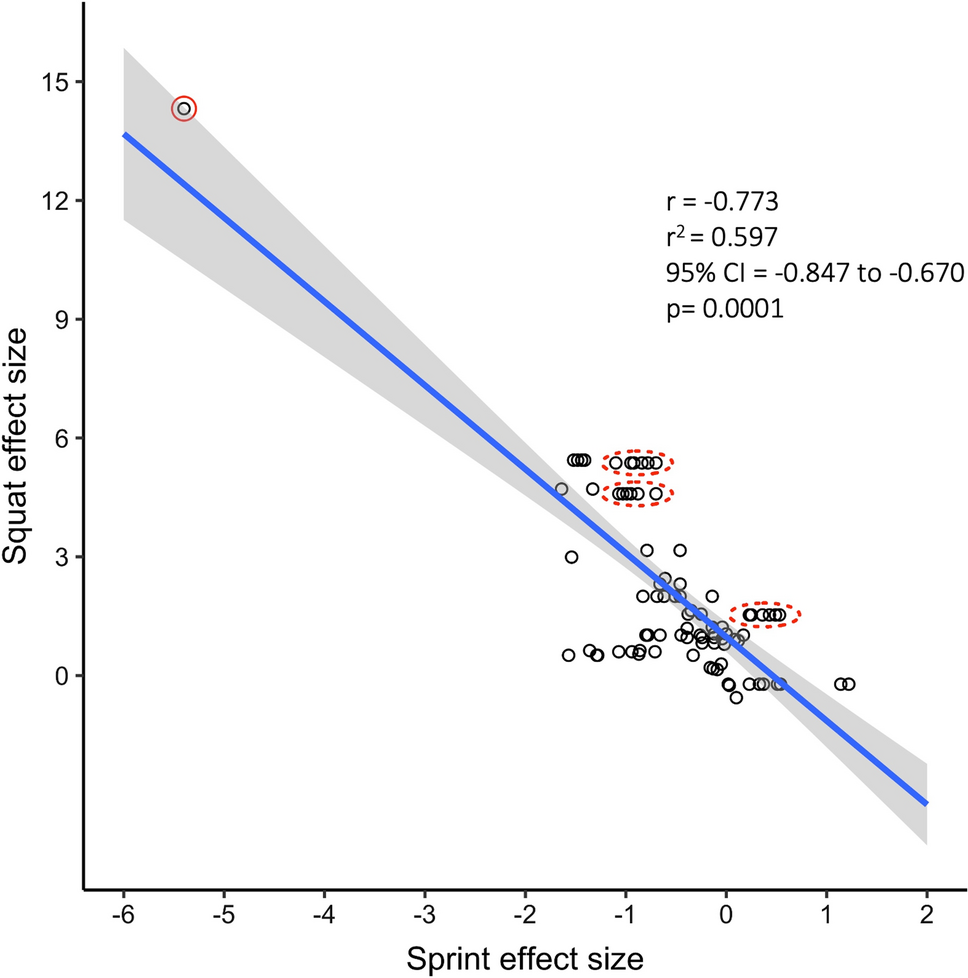
\includegraphics[width=\textwidth]{img/sd_vs_se/kadlec_effect_size.png}
    \caption*{ The most severe over-estimation of effect size made by \href{https://doi.org/10.1007/s40279-014-0227-1}{Seitz et al. (2014)} was for \href{https://doi.org/10.1519/JSC.0b013e3181aa36a2}{Wong et al. (2010)} (solid red circle in the upper right corner of this plot). \href{https://doi.org/10.1007/s40279-022-01766-0}{Kadlec et al. (2022)} corrected the statistical errors made by Seitz et al., finding that Seitz et al. had dramatically overestimated the correlation between lower body strength training and improvement in sprinting performance as a result of these errors. Adapted from Figure 1 of Kadlec et al.}
\end{figure}

\pagebreak

\subsection*{Example 2: Over-weighting studies in a meta-analysis due to using standard error instead of standard deviation}

\href{https://doi.org/10.1016/j.ijcrp.2023.200232}{Garg et al. (2024)} performed a meta-analysis to assess whether the systolic blood pressure was different for groups performing breathing exercises versus not performing breathing exercises at baseline (i.e. before any intervention was applied; note that there is no logical reason to perform this comparison, as it gives no information on the effectiveness of the intervention, but this meta-analysis has numerous issues that are beyond the scope of this guide). For at least two studies, \href{https://doi.org/10.3389/fphys.2020.00898}{Fetter et al. (2020)} and \href{https://doi.org/10.1161/JAHA.121.020980}{Craighead et al. (2021)}, the authors include the standard error as reported by these studies instead of the standard deviation, resulting in these studies being weighted far too heavily.

\begin{figure}[h!tbp]
    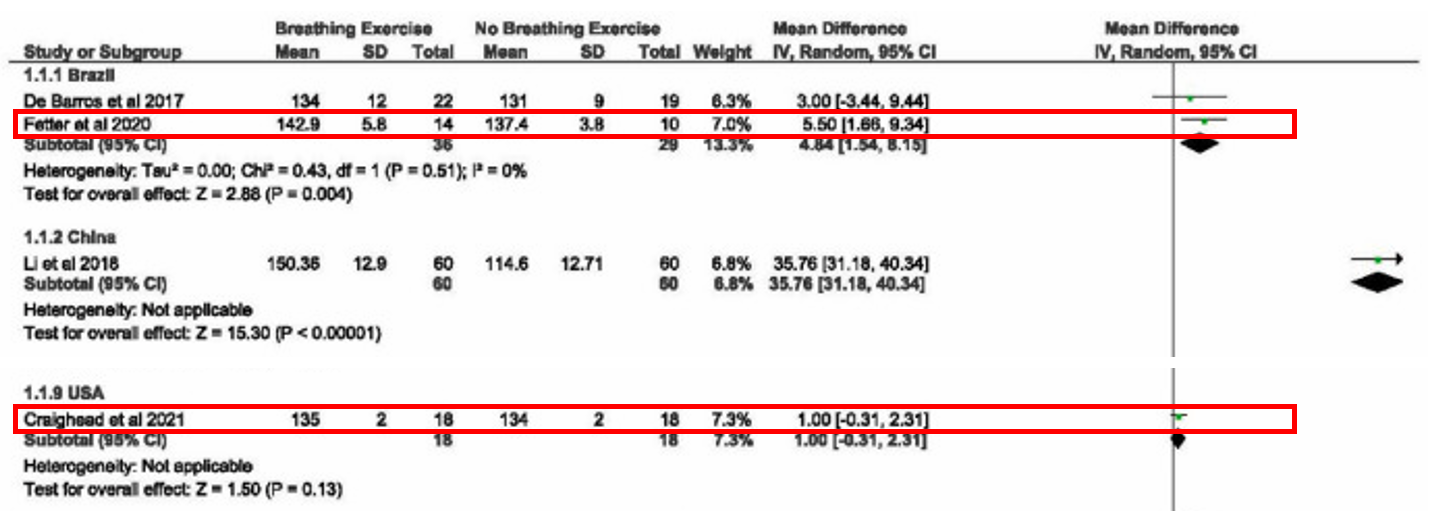
\includegraphics[width=\textwidth]{img/sd_vs_se/garg_problem.PNG}
    \caption*{\href{https://doi.org/10.1016/j.ijcrp.2023.200232}{Garg et al. (2024)} overweighted \href{https://doi.org/10.3389/fphys.2020.00898}{Fetter et al. (2020)} and \href{https://doi.org/10.1161/JAHA.121.020980}{Craighead et al. (2021)} (highlighted in their forest plot in red boxes) as a result of confusing standard error for standard deviation. As a result, Fetter et al. and Craighead et al. are each weighted greater than Li et al. (2018) which had three to four times as many participants. Adapted from Figure 2 of Garg et al.}
\end{figure}

\subsection*{Example 3: Over-weighting studies in a meta-analysis due to using standard error instead of standard deviation}

\href{https://doi.org/10.1007/s11882-023-01085-y}{Chagas et al. (2023)} performed a meta-analysis to determine whether treatment with the drug \href{https://en.wikipedia.org/wiki/Tezepelumab}{tezepelumab} reduced asthma patients' scores on the \href{http://www.qoltech.co.uk/acq.html}{Asthma Control Questionnaire-6 (ACQ-6)}. For the \href{https://doi.org/10.1056/NEJMoa2034975}{NAVIGATOR trial}, the authors entered the reported standard error as the standard deviation, leading to this trial being weighted to 97.6\% for this outcome (meaning that this portion of the meta-analysis was almost entirely based on the results of the NAVIGATOR trial).

\begin{figure}[h!tbp]
    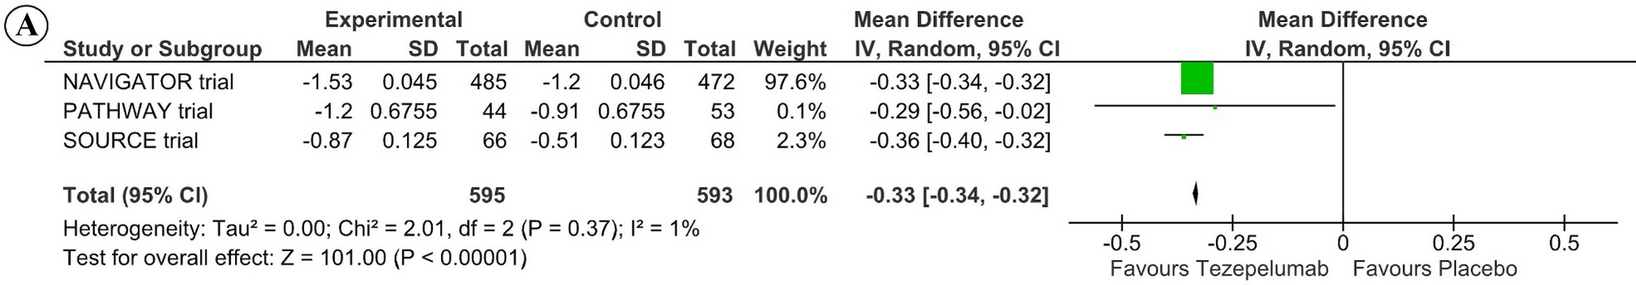
\includegraphics[width=\textwidth]{img/sd_vs_se/chagas_problem.png}
    \caption*{\href{https://doi.org/10.1007/s11882-023-01085-y}{Chagas et al. (2023)} overweighted the \href{https://doi.org/10.1056/NEJMoa2034975}{NAVIGATOR trial} as a result of confusing standard error for standard deviation. Note that the ``standard deviation'' reported in the above forest plot is much lower for the NAVIGATOR trial than the PATHWAY trial or the SOURCE trial. Adapted from Figure 2 of Chagas et al.}
\end{figure}

\pagebreak

\subsection*{Additional resources}

\begin{itemize}
    \setlength\itemsep{-0.5em}
    \item \href{https://doi.org/10.1038/nmeth.2659}{``Points of significance: Error bars'' (2013)}
    \item \href{https://doi.org/10.1007/s40279-023-01989-9}{``The Standard Error/Standard Deviation Mix-Up: Potential Impacts on Meta-Analyses in Sports Medicine'' (2024)}
    \item \href{https://doi.org/10.1007/s40279-022-01766-0}{``With Great Power Comes Great Responsibility: Common Errors in Meta-Analyses and Meta-Regressions in Strength \& Conditioning Research'' (2022)}
    \item \href{https://training.cochrane.org/handbook/current/}{\textit{The Cochrane Handbook for Systematic Reviews of Interventions}}
    \item \href{https://training.cochrane.org/handbook-diagnostic-test-accuracy/current}{\textit{The Cochrane Handbook for Systematic Reviews of Diagnostic Test Accuracy}}

\end{itemize}

% \setlength\itemsep{-0.5em}
% for bullet points and numbered lists.

\end{document}
\documentclass[letterpaper, 12pt]{article}

\usepackage{geometry}
 \geometry{
 letterpaper,
 total={170mm,257mm},
 left=20mm,
 top=20mm,
 bottom=20mm
 }
\usepackage{graphicx} % Required for inserting images
\usepackage{authblk}
\usepackage{amssymb}
\usepackage{lipsum}
\usepackage{float}
\usepackage{times}
\usepackage{amsmath}
\usepackage[format=plain,
            labelfont={bf,it},
            textfont=it]{caption}
\captionsetup{justification=raggedright,singlelinecheck=false}
\usepackage{ragged2e}
\usepackage{longtable}
\usepackage{comment}
\usepackage{setspace}
\usepackage{fancyhdr}
\usepackage{titlesec}
\usepackage[hyperindex,breaklinks]{hyperref}
\hypersetup{
    colorlinks=true,
    linkcolor=blue,
    filecolor=magenta,      
    urlcolor=blue,
    pdftitle={Overleaf Example},
    pdfpagemode=FullScreen,
    }
% \usepackage{background} % add COSIG logo to page
\usepackage[T1]{fontenc}
\usepackage{helvet}
\renewcommand{\familydefault}{\sfdefault}
\pagenumbering{gobble}
\usepackage[skip=10pt plus1pt, indent=40pt]{parskip}

\begin{comment}
\backgroundsetup{
   scale=1,
   angle=0,
   opacity=1,
   color=black,
   contents={\begin{tikzpicture}[remember picture, overlay]
      \node at ([xshift=3cm,yshift=1cm] current page.south west)
            {
\includegraphics[width = 5cm]{img/home/241017_final_logo_mockup.png}}; %<- change the name of image
     \end{tikzpicture}}
 }
\end{comment}

\titlespacing*{\section}
{0pt}{1.5ex plus 1ex minus .2ex}{1.3ex plus .2ex}

\renewcommand\Authfont{\fontsize{12}{14.4}\selectfont}
\renewcommand\Affilfont{\fontsize{9}{10.8}\itshape}
 
\begin{document}
\flushleft

\includegraphics[width=0.5\textwidth]{img/home/241017_final_logo_mockup.png}

\section*{Software for image forensics}
\textit{Last updated: 7 February 2025}

Publication integrity issues often arise from image integrity issues. Performing image forensics is often very useful for taking part in post-publication peer review, especially in fields that frequently use images in scientific articles (e.g., biomedicine).

While many image integrity issues can be spotted by eye, it is often easier and more efficient to use software to automatically spot issues or make issues more visible to readers. This guide is a catalog of tools and software that are commonly used by sleuths.

Here are some factors to consider when using these tools:

\begin{itemize}
    \setlength\itemsep{-0.5em}
    \item \textbf{There can be false positives.} A tool may flag image features that, upon closer manual examination, do not actually indicate any image integrity issues.
    \item \textbf{There can be false negatives.} A tool may not flag image features that are indicative of image integrity issues. For instance, software for detecting image duplications within a figure may miss some duplications that are visible by eye.
    \item \textbf{Tools may not examine all data types.} There can be entire categories of data (including image data) that have been explicitly excluded by the programmers of a tool because they are not yet comfortable with the sensitivity/specificity of their tool for that data type.
    \item \textbf{Analysis may not be reproducible.} Some of these services and software are updated frequently and the current version of a tool may not yield the same results as a previous version.
    \item \textbf{Analysis of the same images in a different format may yield different results.} For example, if one uploads an entire PDF to a duplication detection tool, the tool may yield different results than if individual images are uploaded, even if the individual images and those in the PDF appear identical by eye. Figures in published articles will often be available in multiple resolutions, which can yield differing results. When performing image forensics, it is always preferable to work with the original, full-resolution, uncropped images provided by a study's authors.
    \item \textbf{Tweaking parameters can yield differing results.} Some tools have sensitivity settings that can be changed by the user. Changing these setting may produce different results for the same images.
    \item \textbf{Different tools do different things.} Not every tool described here has the same functionality or use cases as another tool. Another person without access to your tool of choice may not be able to reproduce your analysis.
\end{itemize}

\pagebreak
\subsection*{Software/tools commonly used for image forensics in post-publication peer review:}

\begin{itemize}
    \setlength\itemsep{-0.5em}
    \item \textbf{\href{https://www.adobe.com/products/photoshop.html}{Adobe Photoshop} (subscription-based)}. Photoshop is an image manipulation software that allows users to adjust color levels, adjust brightness and contrast, overlay images and annotate figures among myriad other features. The United States Department of Health and Human Service Office of Research Integrity provides \href{https://ori.hhs.gov/advanced-forensic-actions}{some toolkits} for image forensics with Photoshop.
    \item \textbf{\href{https://www.gimp.org/}{GIMP (the GNU Image Manipulation Program)} (free to use and open-source)}. GIMP is a image manipulation software with most of the same features and functionality as Photoshop but is free to use (and modify).
    \item \textbf{\href{https://imagetwin.ai/}{Imagetwin} (subscription-based)}. Imagetwin is a browser-based service that allows users to upload article PDFs and individual images, which it will then compare against a large database of published images to see if parts of any of the uploaded images have been used previously. It also detects within-document image duplication and splicing of certain images (e.g., \href{https://en.wikipedia.org/wiki/Western_blot}{Western blots}). Users can control the sensitivity of detection on the Results page of a scan.
    \item \textbf{\href{https://www.proofig.com/}{Proofig} (subscription-based)}. Proofig is a browser-based service that allows users to upload article PDFs and individual images, which it will then compare against a large database of published images to see if parts of any of the uploaded images have been used previously. It also detects within-document image duplication.
    \item \textbf{\href{https://github.com/GuidoBartoli/sherloq}{Sherloq } (free to use and open-source)}. Sherloq is a software environment for image forensics that can be installed on Linux and Windows. Users can perform various image transformations that make manipulation more apparent (such as visualizing \href{https://en.wikipedia.org/wiki/Image_gradient}{luminence gradient}) as well as inspect image metadata.
    \item \textbf{\href{https://29a.ch/photo-forensics/}{Forensically} (free to use)}. Forensically is a browser-based service that offers several tools for image forensics, such as clone detection and levels adjustment.
    \item \textbf{\href{https://fotoforensics.com/}{FotoForensics} (free to use)}. FotoForensics is a browser-based service that offers several tools for image forensics, such as \href{https://en.wikipedia.org/wiki/Error_level_analysis}{error level analysis} and metadata inspection.
    \item \textbf{\href{https://www.figcheck.com/imagecheck}{Figcheck} (subscription-based, limited free use)}. Figcheck is a browser-based service that detects within-document image duplication. Each user is limited to uploading 10 images a day.
    \item \textbf{\href{https://sholtodavid.pythonanywhere.com/}{Image Duplication Check (Sholto David)} (free to use)}. This is a browser-based application that allows the user to upload a PDF and scan for within-document image duplication. 
    \item \textbf{\href{https://www.google.com/?olud=}{Google Lens} (free to use)}. Google Lens is an extension of the Google search engine that allows users to upload an image and finding matching and visually-similar images across the web.
\end{itemize}

\end{document}
\documentclass[letterpaper, 12pt]{article}

\usepackage{geometry}
 \geometry{
 letterpaper,
 total={170mm,257mm},
 left=20mm,
 top=20mm,
 bottom=20mm
 }
\usepackage{graphicx} % Required for inserting images
\usepackage{authblk}
\usepackage{amssymb}
\usepackage{lipsum}
\usepackage{float}
\usepackage{times}
\usepackage[format=plain,
            labelfont={bf,it},
            textfont=it]{caption}
\captionsetup{justification=raggedright,singlelinecheck=false}
\usepackage{ragged2e}
\usepackage{longtable}
\usepackage{comment}
\usepackage{setspace}
\usepackage{fancyhdr}
\usepackage{titlesec}
\usepackage[hyperindex,breaklinks]{hyperref}
\hypersetup{
    colorlinks=true,
    linkcolor=blue,
    filecolor=magenta,      
    urlcolor=blue,
    pdftitle={Overleaf Example},
    pdfpagemode=FullScreen,
    }
% \usepackage{background} % add COSIG logo to page
\usepackage[T1]{fontenc}
\usepackage{helvet}
\renewcommand{\familydefault}{\sfdefault}
\pagenumbering{gobble}
\usepackage[skip=10pt plus1pt, indent=40pt]{parskip}

\begin{comment}
\backgroundsetup{
   scale=1,
   angle=0,
   opacity=1,
   color=black,
   contents={\begin{tikzpicture}[remember picture, overlay]
      \node at ([xshift=3cm,yshift=1cm] current page.south west)
            {
\includegraphics[width = 5cm]{img/home/241017_final_logo_mockup.png}}; %<- change the name of image
     \end{tikzpicture}}
 }
\end{comment}

\titlespacing*{\section}
{0pt}{1.5ex plus 1ex minus .2ex}{1.3ex plus .2ex}

\renewcommand\Authfont{\fontsize{12}{14.4}\selectfont}
\renewcommand\Affilfont{\fontsize{9}{10.8}\itshape}
 
\begin{document}
\flushleft

\includegraphics[width=0.5\textwidth]{img/home/241017_final_logo_mockup.png}

\section*{Extracting vector graphics from a PDF}
\textit{Last updated: 5 February 2025}

It is often difficult to tell if two line graphs have shared features from a published figure alone. While the webpage of a scientific article invariable displays these images in raster format (i.e. pixel-based), the PDF version of the article may actually display these images in vector format, meaning that the features of the figure can be more easily magnified and compared.

An easy way to check if a figure in the PDF of a scientific article is in raster format or vector format is to try highlighting the text in the figure with your cursor (e.g. the text that labels the axes of the graph). If the text within the figure can be highlighted, the image is probably in vector format. Consider \href{https://doi.org/10.1007/s12182-020-00439-9}{this article}, for which the figures in the PDF are in vector format, and \href{https://doi.org/10.1016/j.est.2023.109227}{this article}, for which the images in the PDF are in raster format.

\begin{figure}[h!tbp]
    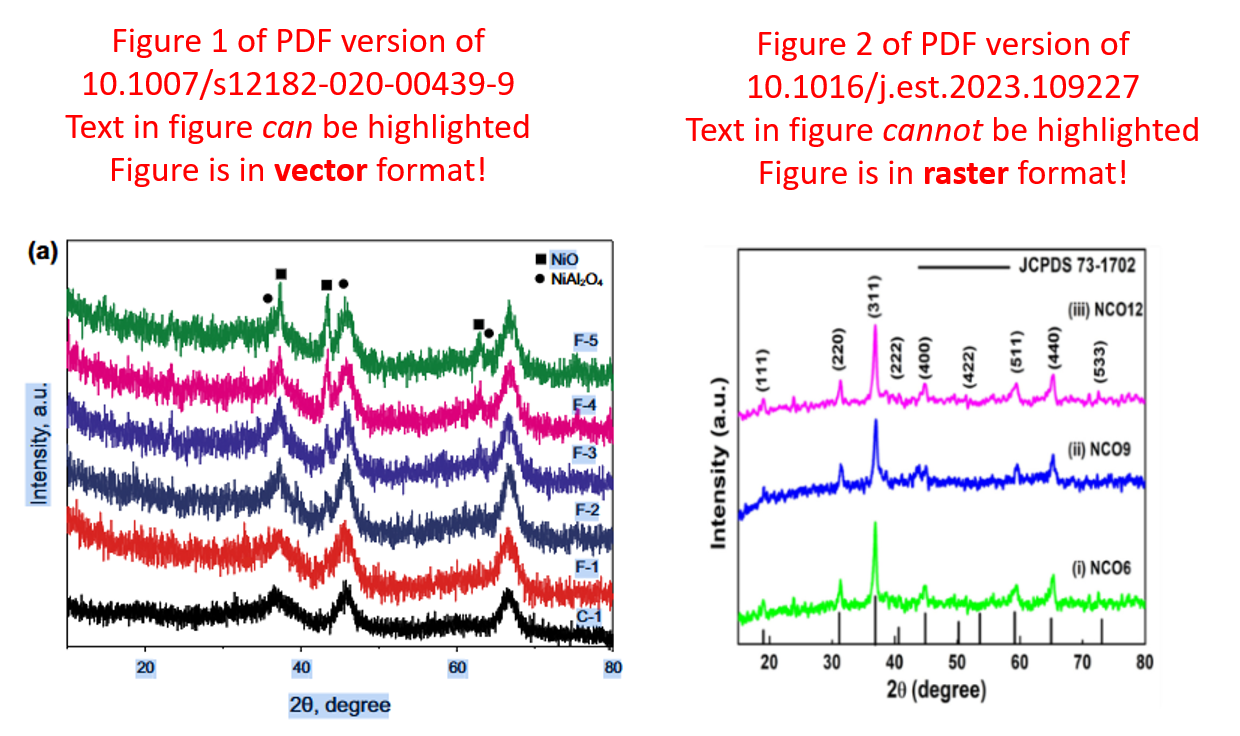
\includegraphics[width=\textwidth]{img/vector/vector_vs_raster.PNG}
    \caption*{ The figure on the left is embedded within its PDF in vector format, whereas the image on the right is embedded within its PDF in raster format.}
\end{figure}

Vector graphics can be isolated in any vector graphics editor like \href{https://www.adobe.com/products/illustrator.html}{Adobe Illustrator} or its free, open-source alternative \href{https://inkscape.org/}{Inkscape}. We'll use Inkscape for this demonstration but the procedure will be more or less the same in other vector graphics editors.

First, open Inkscape, navigate to \textbf{File > Open}, and select your PDF of interest. For this demonstration, we'll use Figure 1B in the PDF of this article. After the PDF opens, scroll over to your figure of interest and select your component of interest.

\begin{figure}[h!tbp]
    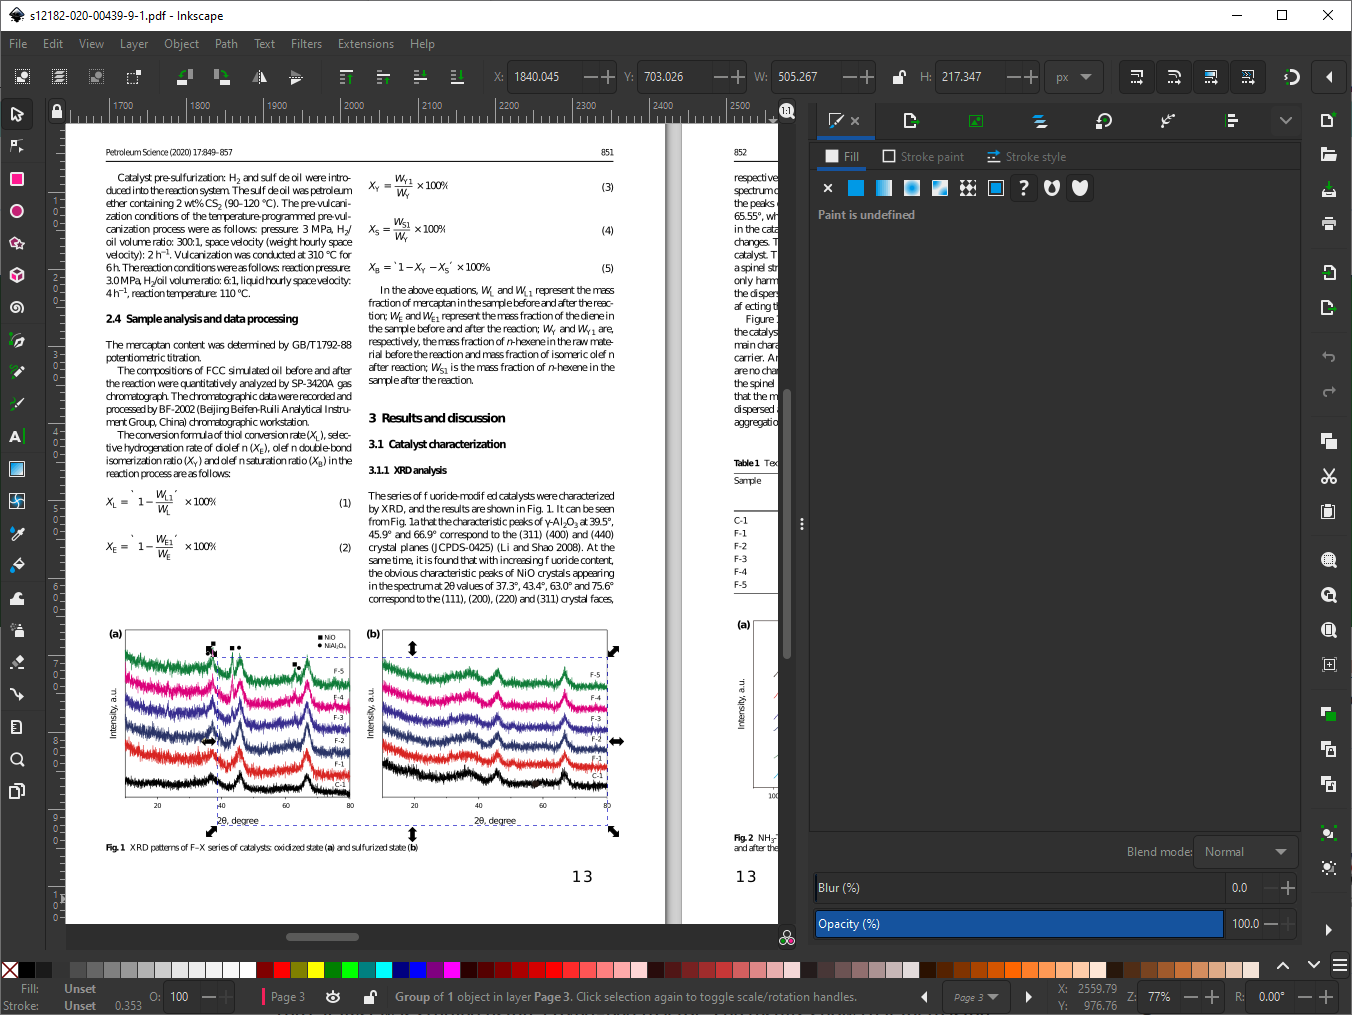
\includegraphics[width=\textwidth]{img/vector/in_inkscape.PNG}
    \caption*{Our PDF opened in Inkscape with the traces in Figure 1B selected.}
\end{figure}

\pagebreak
Next, repeatedly use \textbf{Right click > Ungroup (Shift + Ctrl + G)} on the selected objects until individual objects (in this case, individual line traces) can be selected.

\begin{figure}[h!tbp]
    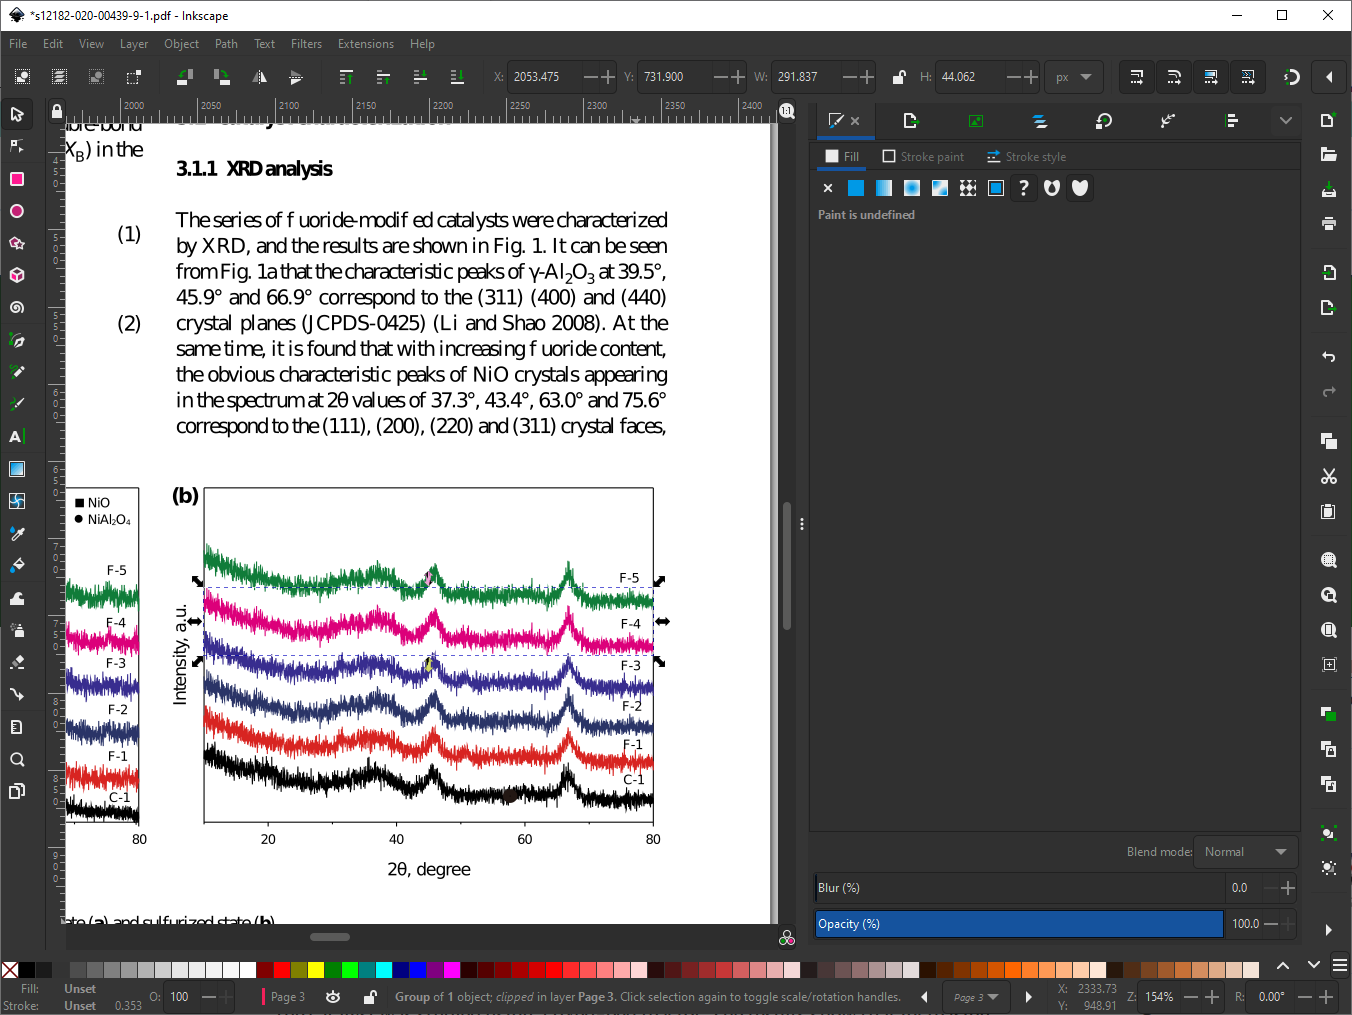
\includegraphics[width=\textwidth]{img/vector/in_inkscape_individual_traces.PNG}
    \caption*{After repeatedly ungrouping objects, we can now select individual line traces.}
\end{figure}

\pagebreak
When viewing line traces, it is helpful, but not necessary, to thin out the traces to enable comparison. To do so, navigate to \textbf{Objects > Fill and Stroke (Shift + Ctrl + F)}, under which the \textbf{Stroke Style} menu allows you to set line thickness. Afterwards, moving the traces to be closer to one another reveals that the F-2 (navy), F-4 (pink) and F-5 (green) traces are identical and the F-3 (blue) and F-1 (red) traces are identical.

\begin{figure}[h!tbp]
    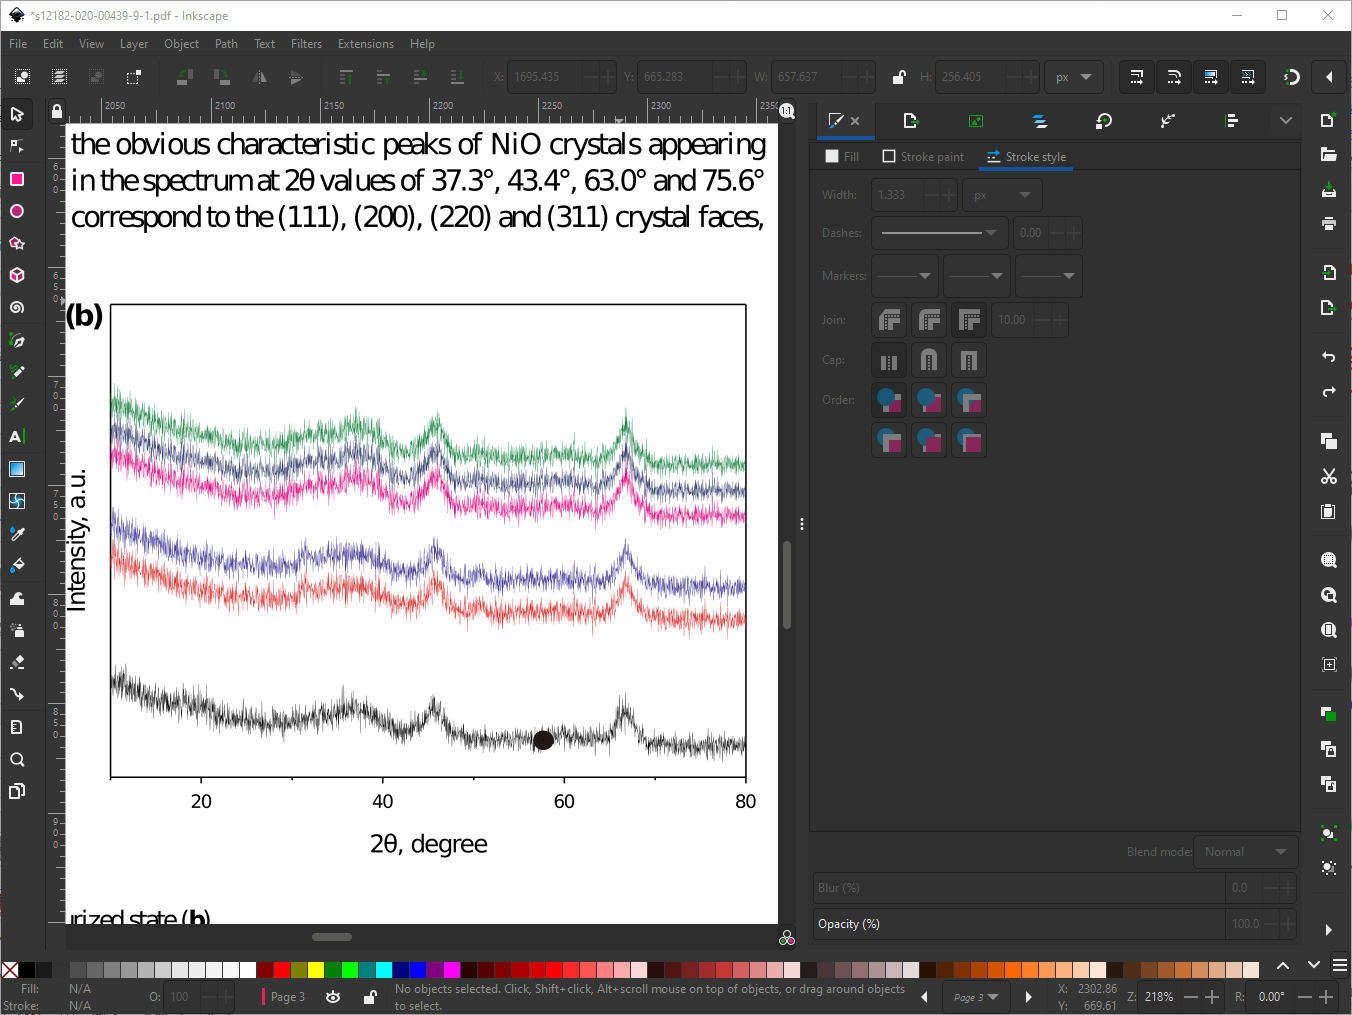
\includegraphics[width=\textwidth]{img/vector/in_inkscape_individual_traces_thinned.PNG}
    \caption*{Moving around and thinning out traces in Inkscape allows for easier comparison.}
\end{figure}

\pagebreak
We can also overlap the traces to make it crystal clear that these are the same data.

\begin{figure}[h!tbp]
    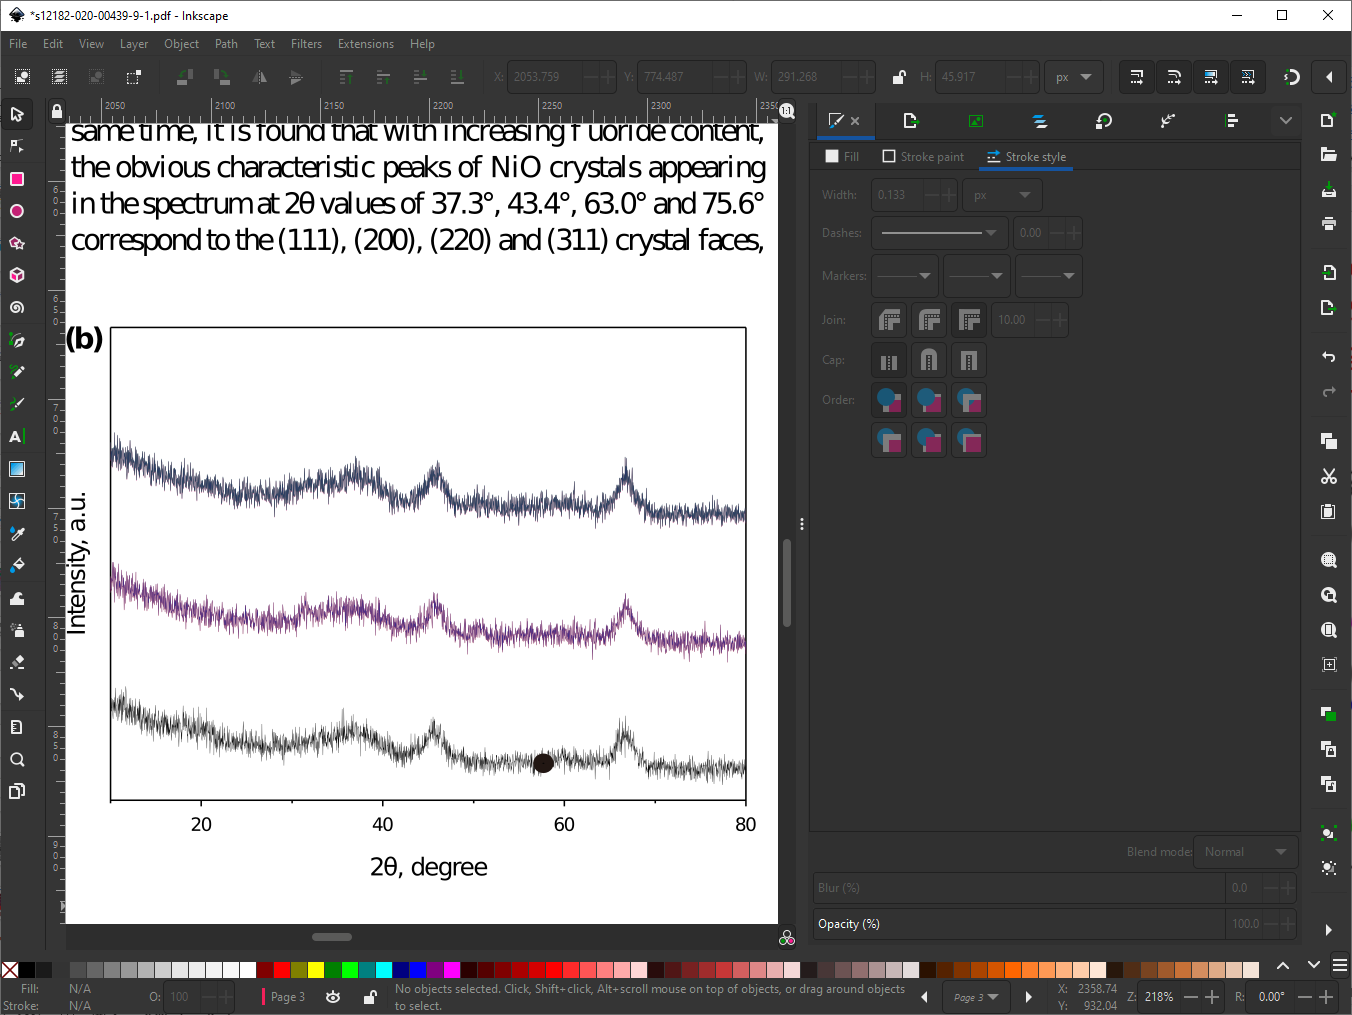
\includegraphics[width=\textwidth]{img/vector/in_inkscape_individual_traces_thinned_overlapping.PNG}
    \caption*{Now that traces are individual objects, we can easily overlap them to show that certain traces are identical.}
\end{figure}

\pagebreak
Objects can also be copy-pasted into a new document.

\begin{figure}[h!tbp]
    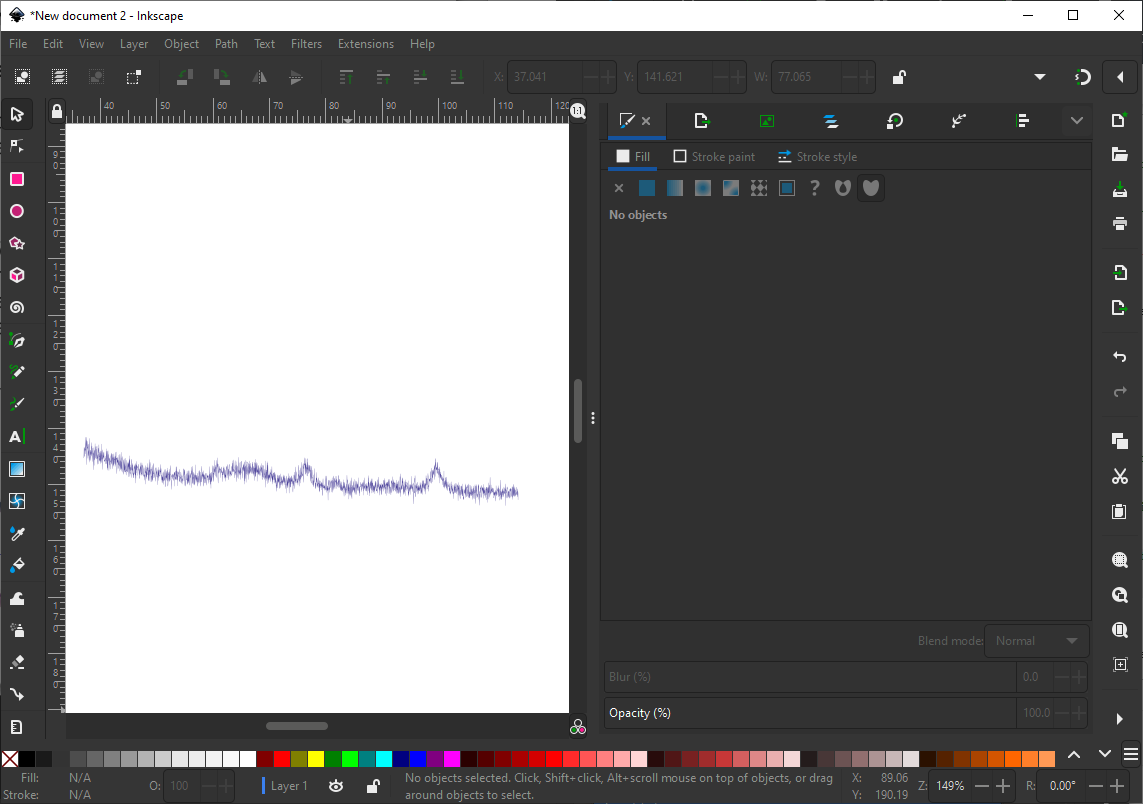
\includegraphics[width=\textwidth]{img/vector/inkscape_new_document.PNG}
    \caption*{ An individual trace copied into a new Inkscape document.}
\end{figure}

\end{document}
\documentclass[letterpaper, 12pt]{article}

\usepackage{geometry}
 \geometry{
 letterpaper,
 total={170mm,257mm},
 left=20mm,
 top=20mm,
 bottom=20mm
 }
\usepackage{graphicx} % Required for inserting images
\usepackage{authblk}
\usepackage{amssymb}
\usepackage{lipsum}
\usepackage{float}
\usepackage{times}
\usepackage{amsmath}
\usepackage[format=plain,
            labelfont={bf,it},
            textfont=it]{caption}
\captionsetup{justification=raggedright,singlelinecheck=false}
\usepackage{ragged2e}
\usepackage{longtable}
\usepackage{comment}
\usepackage{setspace}
\usepackage{fancyhdr}
\usepackage{titlesec}
\usepackage[hyperindex,breaklinks]{hyperref}
\hypersetup{
    colorlinks=true,
    linkcolor=blue,
    filecolor=magenta,      
    urlcolor=blue,
    pdftitle={Overleaf Example},
    pdfpagemode=FullScreen,
    }
% \usepackage{background} % add COSIG logo to page
\usepackage[T1]{fontenc}
\usepackage{helvet}
\renewcommand{\familydefault}{\sfdefault}
\pagenumbering{gobble}
\usepackage[skip=10pt plus1pt, indent=40pt]{parskip}

\begin{comment}
\backgroundsetup{
   scale=1,
   angle=0,
   opacity=1,
   color=black,
   contents={\begin{tikzpicture}[remember picture, overlay]
      \node at ([xshift=3cm,yshift=1cm] current page.south west)
            {
\includegraphics[width = 5cm]{img/home/241017_final_logo_mockup.png}}; %<- change the name of image
     \end{tikzpicture}}
 }
\end{comment}

\titlespacing*{\section}
{0pt}{1.5ex plus 1ex minus .2ex}{1.3ex plus .2ex}

\renewcommand\Authfont{\fontsize{12}{14.4}\selectfont}
\renewcommand\Affilfont{\fontsize{9}{10.8}\itshape}
 
\begin{document}
\flushleft

\includegraphics[width=0.5\textwidth]{img/home/241017_final_logo_mockup.png}

\section*{The vertical line test}
\addcontentsline{toc}{section}{The vertical line test}
\textit{Last updated: 7 February 2025}

For many types of data plotted on a x/y plane, it is expected that each x-axis value maps uniquely to a y-axis value. For instance, if you plotted your height over time, you would expect that each x-axis value (a point in time) corresponds to a single y-axis value (your height at that time). If not, this plot would imply that there were some points in your life where you were two different heights at the same time.

This property defines a \href{https://en.wikipedia.org/wiki/Graph_of_a_function}{mathematical function}, for which there is one unique output (y) for every unique input (x). The \href{https://en.wikipedia.org/wiki/Vertical_line_test}{vertical line test} is a simple method for gauging if a trace/curve is a function or not: given a trace/curve on an x/y plane, can you draw a vertical line that intersects the trace/curve multiple times? If there is at least one such vertical line, the trace/curve is not a mathematical function and may not make sense for the type of data it is describing.

\begin{figure}[h!tbp]
    \centering
    \includegraphics[width=\textwidth]{img/vertical_line/vertical_line_test_mockup.png}
    \caption*{If you plotted your height over time, you would expect each point in time (i.e., each point on the x axis) to correspond to a single height (i.e., a single point on the y axis). The graph on the left matches this expectation and is realistic for this kind of data. The graph in the middle does not match this expectation; there are some points in time that correspond to multiple heights. The graph on the right shows this trace failing the the vertical line test. This is just one of many vertical lines that could be drawn that show that this trace is not a function and thus does not realistically describe data representing height over time.}
\end{figure}

\pagebreak

\subsection*{Data types that should always pass the vertical line test}

Some data types, when plotted, will invariably be functions and thus should always pass the vertical line test. For instance, taking the absorption spectrum of a material should yield one value for absorption for every wavelength. Data types that are always expected to pass the vertical line test include, but are not limited to:

\begin{itemize}
    \setlength\itemsep{-0.5em}
    \item any \href{https://en.wikipedia.org/wiki/Absorption_spectroscopy}{light absorption spectrum}, including ultraviolet-visible (UV-VIS) absorption spectra, infrared (IR) absorption spectra, microwave absorption spectra, X-ray absorption spectra (XAS), etc. (\textit{Note that essentially anything that gets called a ``spectrum" should pass the vertical line test.})
    \item \href{https://en.wikipedia.org/wiki/Nuclear_magnetic_resonance_spectroscopy}{nuclear magnetic resonance (NMR)} spectra
    \item \href{https://en.wikipedia.org/wiki/Electron_paramagnetic_resonance}{electron spin resonance (ESR)/electron paramagnetic resonance (ESR)} spectra
    \item \href{https://en.wikipedia.org/wiki/Fourier-transform_infrared_spectroscopy}{Fourier-transform infrared (FTIR)} spectra
    \item \href{https://en.wikipedia.org/wiki/Raman_spectroscopy}{Raman} spectra
    \item \href{https://en.wikipedia.org/wiki/X-ray_diffraction}{X-ray diffraction (XRD)} patterns/diffractograms
    \item \href{https://en.wikipedia.org/wiki/Energy-dispersive_X-ray_spectroscopy}{energy-dispersive X-ray (EDX/EDS/EDAX)} spectra
    \item \href{https://en.wikipedia.org/wiki/X-ray_photoelectron_spectroscopy}{X-ray photoelectron} spectra (XPS)
    \item \href{https://en.wikipedia.org/wiki/Photoluminescence}{photoluminescence (PL)} spectra
    \item \href{https://en.wikipedia.org/wiki/Mass_spectrometry}{Mass spectra (MS/mass spec)}
    \item \href{https://en.wikipedia.org/wiki/Differential_thermal_analysis}{differential thermal analysis (DTA)} curves
    \item \href{https://en.wikipedia.org/wiki/Differential_scanning_calorimetry}{differential scanning calorimetry (DSC)} curves
    \item \href{https://en.wikipedia.org/wiki/Thermogravimetric_analysis}{thermogravimetric analysis (TGA)}curves
    \item \href{https://en.wikipedia.org/wiki/Transient_photocurrent}{photocurrent response/transient photocurrent (TPC)} curves
    \item \href{https://en.wikipedia.org/wiki/Electroencephalography}{electroencephalograms (EEG)}
    \item \href{https://en.wikipedia.org/wiki/Patch_clamp}{patch-clamp} recordings
\end{itemize}

\subsection*{Data types that may not pass the vertical line test}

For some data types, it is entirely expected that some x axis values will map to multiple y axis values. Data types that may or may not pass the vertical line test include, but are not limited to:

\begin{itemize}
    \setlength\itemsep{-0.5em}
    \item \href{https://en.wikipedia.org/wiki/Cyclic_voltammetry}{cyclic voltammetry (CV)} curves
    \item traces of an object moving in two dimensions, such as a mouse solving a \href{https://en.wikipedia.org/wiki/Morris_water_navigation_task}{Morris water navigation task}
    \item \href{https://en.wikipedia.org/wiki/Pressure%E2%80%93volume_diagram}{Pressure-volume (PV) diagrams}
    \item diagrams of \href{https://en.wikipedia.org/wiki/Graph_theory}{mathematical graphs/networks}
\end{itemize}

\pagebreak

\subsection*{Example 1: Passes the vertical line test}

\href{https://doi.org/10.1021/acsami.4c03997}{Thomas et al. (2024)} report using X-ray diffraction (XRD), Fourier-transform infrared spectroscopy (FTIR) and thermogravimetric analysis (TGA), among other techniques, to characterize kaolinite and kaolinite nanoplatelets. Each of these techniques yield data with one value on the y axis for each value on the x axis. All the plots corresponding to these techniques provided by Thomas et al. pass the vertical line test, as expected.

\begin{figure}[h!tbp]
    \centering
    \includegraphics[width=\textwidth]{img/vertical_line/thomas_et_al_mockup.png}
    \caption*{Plots from \href{https://doi.org/10.1021/acsami.4c03997}{Thomas et al. (2024)} that pass the vertical line test (adapted from Figures 2B, S8 and S2).}
\end{figure}

\subsection*{Example 2: Does not pass the vertical line test}

\href{https://doi.org/10.1016/j.ceramint.2014.07.091}{Mandizadeh et al. (2014)} report using FTIR to characterize barium hexaferrite nanostructures. However, the FTIR spectrum they show backtracks on itself several times, failing the vertical line test.

\begin{figure}[h!tbp]
    \centering
    \includegraphics[width=0.6\textwidth]{img/vertical_line/mandizaeh_ftir.png}
    \caption*{An FTIR spectrum from Figure 1 of \href{https://doi.org/10.1016/j.ceramint.2014.07.091}{Mandizadeh et al. (2014)} that fails the vertical line test.}
\end{figure}

\pagebreak

\subsection*{Example 3: Does not pass the vertical line test}

\href{https://doi.org/10.1007/s10854-024-13064-8}{Suguna et al. (2024)} report using FTIR to characterize nanocomposite photocatalysts. However, the FTIR spectra they show appear to be hand-drawn and some fail the vertical line test.

\begin{figure}[h!tbp]
    \centering
    \includegraphics[width=\textwidth]{img/vertical_line/suguna_ftir.png}
    \caption*{FTIR spectra from Figure 3A \href{https://doi.org/10.1007/s10854-024-13064-8}{Suguna et al. (2024)}. The ZnFe$_2$O$_4$ spectrum (in blue) fails the vertical line test.}
\end{figure}

\pagebreak

\subsection*{Example 4: Vertical line test does not apply}

\href{https://doi.org/10.1371/journal.pcbi.1004110}{Lepora and Pezzulo (2015)} describe tracking mice in 2D space. They include several mouse trajectories in figures which follow the path of a mouse with a line. These trajectories are not expected to be functions and thus the vertical line test does not apply.

\begin{figure}[h!tbp]
    \centering
    \includegraphics[width=\textwidth]{img/vertical_line/pcbi.1004110.g002.png}
    \caption*{Mouse trajectory traces in 2D space, for which the vertical line test does not apply. Adapted from Figure 2 of \href{https://doi.org/10.1371/journal.pcbi.1004110}{Lepora and Pezzulo (2015)}.}
\end{figure}


\end{document}
\documentclass[letterpaper, 12pt]{article}

\usepackage{geometry}
 \geometry{
 letterpaper,
 total={170mm,257mm},
 left=20mm,
 top=20mm,
 bottom=20mm
 }
\usepackage{graphicx} % Required for inserting images
\usepackage{authblk}
\usepackage{amssymb}
\usepackage{lipsum}
\usepackage{float}
\usepackage{times}
\usepackage{amsmath}
\usepackage[format=plain,
            labelfont={bf,it},
            textfont=it]{caption}
\captionsetup{justification=raggedright,singlelinecheck=false}
\usepackage{ragged2e}
\usepackage{longtable}
\usepackage{comment}
\usepackage{setspace}
\usepackage{fancyhdr}
\usepackage{titlesec}
\usepackage[hyperindex,breaklinks]{hyperref}
\hypersetup{
    colorlinks=true,
    linkcolor=blue,
    filecolor=magenta,      
    urlcolor=blue,
    pdftitle={Overleaf Example},
    pdfpagemode=FullScreen,
    }
% \usepackage{background} % add COSIG logo to page
\usepackage[T1]{fontenc}
\usepackage{helvet}
\renewcommand{\familydefault}{\sfdefault}
\pagenumbering{gobble}
\usepackage[skip=10pt plus1pt, indent=40pt]{parskip}

\begin{comment}
\backgroundsetup{
   scale=1,
   angle=0,
   opacity=1,
   color=black,
   contents={\begin{tikzpicture}[remember picture, overlay]
      \node at ([xshift=3cm,yshift=1cm] current page.south west)
            {\includegraphics[width = 5cm]{img/home/241017_final_logo_mockup.png}}; %<- change the name of image
     \end{tikzpicture}}
 }
\end{comment}

\titlespacing*{\section}
{0pt}{1.5ex plus 1ex minus .2ex}{1.3ex plus .2ex}

\renewcommand\Authfont{\fontsize{12}{14.4}\selectfont}
\renewcommand\Affilfont{\fontsize{9}{10.8}\itshape}
 
\begin{document}
\flushleft
\includegraphics[width=0.5\textwidth]{img/home/241017_final_logo_mockup.png}

\section*{X-ray diffraction patterns - Scherrer's equation}
\textit{Last updated: 6 February 2025}

\subsection*{X-ray diffraction patterns/diffractograms}

\href{https://web.pdx.edu/~pmoeck/phy381/Topic5a-XRD.pdf}{X-ray diffraction (XRD)} is a popular experimental technique used to characterize the nanoscale structure of materials like crystals, glasses and even liquids. XRD involves bombarding a sample with high-energy X-rays at a range of incident angles.

For a material with some amount of repetitive atomic structure, the reflected X-rays will have higher intensity at specific angles (``peaks'') corresponding to the distance between successive layers of atoms.

A typical graph of an XRD pattern will have intensity of signal on the y axis and the \href{https://en.wikipedia.org/wiki/Bragg%27s_law}{Bragg angle} $\theta$
(expressed as $2\theta$ by convention) on the x axis. Peaks may be labeled with the \href{https://chem.libretexts.org/Courses/Lafayette_College/CHEM_212_213%3A_Inorganic_Chemistry_(Nataro)/03%3A_Solid_state/3.10%3A_Miller_Indices_(hkl)}{Miller indices} of the corresponding crystal plane.

\begin{figure}[h!tbp]
    \includegraphics[width=\textwidth]{img/xrd/powder__2857__1486.png}
    \caption*{An example XRD pattern for the mineral \href{https://rruff.info/R061069}{Hibonite}.}
\end{figure}

Solids may be described as amorphous (having no discernable long-range ordering of atoms), polycrystalline (having long-range ordering, but only within small domains) or crystalline (being made up of one large crystalline domain). Generally, materials with a more ordered structure will yield XRD patterns with sharper peaks. Thus, crystalline materials will tend to yield XRD patterns with very sharp, needle-like peaks, polycrystalline materials will tend to yield XRD patterns with somewhat broader, mountain-like peaks and amorphous materials will tend to yield XRD patterns with very broad, hill-like peaks.

\begin{figure}[h!tbp]
    \includegraphics[width=\textwidth]{img/xrd/xrd_mockup.jpg}
    \caption*{ Materials with large crystalline domains will tend have very sharp peaks, whereas a material with no crystalline domains will tend to have very broad peaks. Note that these XRD patterns are hand-drawn to demonstrate peak broadening and do not correspond to any real material. Images adapted from \href{https://alan.ece.gatech.edu/ECE3040/Lectures/Lecture1-ElectronicMaterialsPierretChap1and2.pdf}{lecture notes of Dr. Alan Doolittle.}}
\end{figure}

\subsection*{Crystallites, grains and particles}

\href{https://www.eng.uc.edu/~beaucag/Classes/Properties%20of%20Materials/MITCrystalSizeAnalysis.pdf}{Crystallite size} describes the typical size of crystalline domains that scatter X-rays coherently (i.e., regions of the solid where the crystal lattice is all oriented the same way). \href{https://doi.org/10.1088/0957-4484/21/14/145701}{Grain size} has a similar definition, also referring to the typical size of regions of the solid where the crystal is oriented in the same direction. However, grain size is usually estimated from \href{https://en.wikipedia.org/wiki/High-resolution_transmission_electron_microscopy}{high resolution transmission electron microscopy} images and crystallite size is usually estimated from XRD patterns. A grain can be made up of a single crystallite or multiple crystallites. `Grain' and `crystallite' are often used interchangeably.

$$ \text{crystallite size} \leq \text{grain size} \leq \text{particle size}$$

\subsection*{Scherrer's equation}

\href{}{Scherrer's equation} (sometimes called the Scherrer relation or the Debye-Scherrer equation, though \href{https://doi.org/10.1038/nnano.2011.145}{not without controversy}) is a formula for estimating the mean crystallite size within a material based on the width of peaks in its XRD pattern. For a mean crystallite size of $D$, Scherrer's equation is

$$ D = \frac{K \lambda}{\beta \cos \theta} $$

where $K$ is a dimensionless shape factor (usually taken as 0.89, 0.94 or 1.0, \href{https://doi.org/10.1107/S0021889878012844}{depending on the shape of the crystal}), $\lambda$ is the wavelength of the X-rays used (usually 1.5406 \r{A}), $\beta$ is the \href{https://en.wikipedia.org/wiki/Full_width_at_half_maximum}{full width at half-maximum} of the peak in being used (in radians) and $\theta$ is the Bragg angle (in radians). Usually $D$ is estimated using only the tallest peak in the pattern. Full width at half maximum (FWHM) describes the width of the peak at the point halfway between the bottom of the peak and the top of the peak and is usually measured by fitting peaks with a Gaussian curve in software.

For assessing the integrity of crystallite size estimates made in an article using Scherrer's equation, there are three important details to note:

\begin{enumerate}
    \setlength\itemsep{-0.5em}
    \item $D$ is inversely proportional to $\beta$. In other words, as peaks become wider, crystallite sizes decrease; as peaks become narrower, crystallite sizes increase.
    \item Scherrer's equation is used for estimating crystallite size, \textit{not} particle size.
    \item Crystallite size must always be smaller than or equal to particle size.
\end{enumerate}

\subsection*{Example 1: No detectable integrity issues concerning Scherrer's equation}

In \href{https://10.0.4.64/2043-6254/ab52f7}{Mustapha et al. (2019)}, the authors use Scherrer's equation to estimate crystallite size of ZnO nanoparticles synthesized at varying pH. The XRD patterns shown in Figure 2 are consistent with the the calculated crystallite sizes shown in Table 1. Observe that as peaks become wider from pattern (a) to pattern (e), crystallite size decreases. There is nothing unexpected here. 

\begin{figure}[h!tbp]
    \includegraphics[width=\textwidth]{img/xrd/xrd_publication_mockup_mustapha.jpg}
    \caption*{Adapted from Figure 1 and Table 1 of \href{https://10.0.4.64/2043-6254/ab52f7}{Mustapha et al. (2019)}.}
\end{figure}

\subsection*{Example 2: Unexpected results from Scherrer's equation, inconsistency between particle sizes and crystallite sizes}

In \href{https://doi.org/10.3390/nano9071024}{Khan et al. (2019)}, the authors use Scherrer's equation to estimate crystallite sizes for Ni- and Zn-based nanoferrites. The authors state:

\begin{quote}
    \textit{The Scherrer formula is used to evaluate the particle size using the extreme intense peak (311). The experimental results demonstrate that precipitated particles’ size was in the range of 20–60 nm.}
\end{quote}

Recall that Scherrer's equation is used to estimate crystallite size, not particle size. Moreover, the authors' claimed crystallite sizes shown in Figure 2B and Table 1 imply that the (311) peak should be about three times as wide for X = 0 than X = 1. However, in Figure 2A, no such peak broadening is present in the XRD patterns shown. If anything, the (311) peak is wider for X = 1 than X = 0. 

\begin{figure}[h!tbp]
    \includegraphics[width=0.8\textwidth]{img/xrd/xrd_publication_mockup_khan.jpg}
    \caption*{ Adapted from Figure 2A and Figure 2B of \href{https://doi.org/10.3390/nano9071024}{Khan et al. (2019)}.}
\end{figure}

Finally, some of the claimed crystallite sizes are larger than the nanoparticles shown for the same materials in the SEM images in Figure 1. 

\begin{figure}[h!tbp]
\centering
    \includegraphics[width=0.8\textwidth]{img/xrd/xrd_sem_images_khan.jpg}
    \caption*{ Adapted from Figure 1 of \href{https://doi.org/10.3390/nano9071024}{Khan et al. (2019)}.}
\end{figure}

\subsection*{Example 3: Unexpected results from Scherrer's equation}

In \href{https://doi.org/10.1021/acs.energyfuels.2c03279}{Abdullah et al. (2023)}, the authors use Scherrer's equation to estimate crystallite sizes of AgTe nanostructures. They state:

\begin{quote}
    \textit{Effect of Ag0.006Te, Ag0.012Te, Ag0.025Te, Ag0.05Te, and Ag0.1Te nanostructure was determined with crystallite size found in the range of 85 nm, 73 nm and 39 nm, and 67 nm and 88 nm, respectively, measured with Debye Scherer.}
\end{quote}

If the crystallite size of Ag0.025Te is twice as small as its counterparts, one would expect the peaks in the XRD pattern for Ag0.025Te to be twice as wide. However, this is not observed in the XRD patterns shown in Figure 1A. In fact, the patterns shown for all materials in Figure 1A are identical except for vertical scaling.

\begin{figure}[h!tbp]
\centering
    \includegraphics[width=0.7\textwidth]{img/xrd/xrd_spectra_abdullah.png}
    \caption*{ Adapted from Figure 1A of \href{https://doi.org/10.1021/acs.energyfuels.2c03279}{Abdullah et al. (2023)}.}
\end{figure}

\subsection*{Example 4: confusion of crystallite size with particle size}

In \href{https://doi.org/10.1016/j.jallcom.2016.03.279}{Upadhyay et al. (2016)}, the authors use Scherrer's equation to estimate crystallite sizes of magnetite nanoparticles. However, throughout the article the authors refer to crystallite size and particle size interchangeably, several times claiming that particle size can be determined by Scherrer's equation. For instace, the caption of Table 1 reads:

\begin{quote}
    \textit{Table 1. Particle size, lattice parameter and strain in the sample calculated from X-ray data. Size (S) represent particle/crystallite size calculated using Scherer formula while Size (WH) represent particle/crystallite size calculated from Williamson–Hall method.}
\end{quote}

\end{document}

\end{document}